\documentclass[twoside]{book}

% Packages required by doxygen
\usepackage{fixltx2e}
\usepackage{calc}
\usepackage{doxygen}
\usepackage[export]{adjustbox} % also loads graphicx
\usepackage{graphicx}
\usepackage[utf8]{inputenc}
\usepackage{makeidx}
\usepackage{multicol}
\usepackage{multirow}
\PassOptionsToPackage{warn}{textcomp}
\usepackage{textcomp}
\usepackage[nointegrals]{wasysym}
\usepackage[table]{xcolor}

% Font selection
\usepackage[T1]{fontenc}
\usepackage[scaled=.90]{helvet}
\usepackage{courier}
\usepackage{amssymb}
\usepackage{sectsty}
\renewcommand{\familydefault}{\sfdefault}
\allsectionsfont{%
  \fontseries{bc}\selectfont%
  \color{darkgray}%
}
\renewcommand{\DoxyLabelFont}{%
  \fontseries{bc}\selectfont%
  \color{darkgray}%
}
\newcommand{\+}{\discretionary{\mbox{\scriptsize$\hookleftarrow$}}{}{}}

% Page & text layout
\usepackage{geometry}
\geometry{%
  a4paper,%
  top=2.5cm,%
  bottom=2.5cm,%
  left=2.5cm,%
  right=2.5cm%
}
\tolerance=750
\hfuzz=15pt
\hbadness=750
\setlength{\emergencystretch}{15pt}
\setlength{\parindent}{0cm}
\setlength{\parskip}{3ex plus 2ex minus 2ex}
\makeatletter
\renewcommand{\paragraph}{%
  \@startsection{paragraph}{4}{0ex}{-1.0ex}{1.0ex}{%
    \normalfont\normalsize\bfseries\SS@parafont%
  }%
}
\renewcommand{\subparagraph}{%
  \@startsection{subparagraph}{5}{0ex}{-1.0ex}{1.0ex}{%
    \normalfont\normalsize\bfseries\SS@subparafont%
  }%
}
\makeatother

% Headers & footers
\usepackage{fancyhdr}
\pagestyle{fancyplain}
\fancyhead[LE]{\fancyplain{}{\bfseries\thepage}}
\fancyhead[CE]{\fancyplain{}{}}
\fancyhead[RE]{\fancyplain{}{\bfseries\leftmark}}
\fancyhead[LO]{\fancyplain{}{\bfseries\rightmark}}
\fancyhead[CO]{\fancyplain{}{}}
\fancyhead[RO]{\fancyplain{}{\bfseries\thepage}}
\fancyfoot[LE]{\fancyplain{}{}}
\fancyfoot[CE]{\fancyplain{}{}}
\fancyfoot[RE]{\fancyplain{}{\bfseries\scriptsize Generated by Doxygen }}
\fancyfoot[LO]{\fancyplain{}{\bfseries\scriptsize Generated by Doxygen }}
\fancyfoot[CO]{\fancyplain{}{}}
\fancyfoot[RO]{\fancyplain{}{}}
\renewcommand{\footrulewidth}{0.4pt}
\renewcommand{\chaptermark}[1]{%
  \markboth{#1}{}%
}
\renewcommand{\sectionmark}[1]{%
  \markright{\thesection\ #1}%
}

% Indices & bibliography
\usepackage{natbib}
\usepackage[titles]{tocloft}
\setcounter{tocdepth}{3}
\setcounter{secnumdepth}{5}
\makeindex

% Hyperlinks (required, but should be loaded last)
\usepackage{ifpdf}
\ifpdf
  \usepackage[pdftex,pagebackref=true]{hyperref}
\else
  \usepackage[ps2pdf,pagebackref=true]{hyperref}
\fi
\hypersetup{%
  colorlinks=true,%
  linkcolor=blue,%
  citecolor=blue,%
  unicode%
}

% Custom commands
\newcommand{\clearemptydoublepage}{%
  \newpage{\pagestyle{empty}\cleardoublepage}%
}

\usepackage{caption}
\captionsetup{labelsep=space,justification=centering,font={bf},singlelinecheck=off,skip=4pt,position=top}

%===== C O N T E N T S =====

\begin{document}

% Titlepage & ToC
\hypersetup{pageanchor=false,
             bookmarksnumbered=true,
             pdfencoding=unicode
            }
\pagenumbering{alph}
\begin{titlepage}
\vspace*{7cm}
\begin{center}%
{\Large World Imaker }\\
\vspace*{1cm}
{\large Generated by Doxygen 1.8.13}\\
\end{center}
\end{titlepage}
\clearemptydoublepage
\pagenumbering{roman}
\tableofcontents
\clearemptydoublepage
\pagenumbering{arabic}
\hypersetup{pageanchor=true}

%--- Begin generated contents ---
\chapter{Namespace Index}
\section{Namespace List}
Here is a list of all documented namespaces with brief descriptions\+:\begin{DoxyCompactList}
\item\contentsline{section}{\hyperlink{namespaceglimac}{glimac} \\*Outils de gestion d\textquotesingle{}une scène 3D }{\pageref{namespaceglimac}}{}
\end{DoxyCompactList}

\chapter{Hierarchical Index}
\section{Class Hierarchy}
This inheritance list is sorted roughly, but not completely, alphabetically\+:\begin{DoxyCompactList}
\item \contentsline{section}{glimac\+:\+:Controls}{\pageref{classglimac_1_1Controls}}{}
\item \contentsline{section}{glimac\+:\+:Cube}{\pageref{classglimac_1_1Cube}}{}
\item \contentsline{section}{glimac\+:\+:Cube\+List}{\pageref{classglimac_1_1CubeList}}{}
\item \contentsline{section}{glimac\+:\+:File\+Path}{\pageref{classglimac_1_1FilePath}}{}
\item \contentsline{section}{std\+:\+:hash$<$ glimac\+:\+:File\+Path $>$}{\pageref{structstd_1_1hash_3_01glimac_1_1FilePath_01_4}}{}
\item \contentsline{section}{glimac\+:\+:Image}{\pageref{classglimac_1_1Image}}{}
\item \contentsline{section}{glimac\+:\+:Image\+Manager}{\pageref{classglimac_1_1ImageManager}}{}
\item \contentsline{section}{tinyobj\+:\+:material\+\_\+t}{\pageref{structtinyobj_1_1material__t}}{}
\item \contentsline{section}{tinyobj\+:\+:Material\+Reader}{\pageref{classtinyobj_1_1MaterialReader}}{}
\begin{DoxyCompactList}
\item \contentsline{section}{tinyobj\+:\+:Material\+File\+Reader}{\pageref{classtinyobj_1_1MaterialFileReader}}{}
\end{DoxyCompactList}
\item \contentsline{section}{tinyobj\+:\+:mesh\+\_\+t}{\pageref{structtinyobj_1_1mesh__t}}{}
\item \contentsline{section}{tinyobj\+:\+:obj\+\_\+shape}{\pageref{structtinyobj_1_1obj__shape}}{}
\item \contentsline{section}{glimac\+:\+:Program}{\pageref{classglimac_1_1Program}}{}
\item \contentsline{section}{glimac\+:\+:S\+D\+L\+Window\+Manager}{\pageref{classglimac_1_1SDLWindowManager}}{}
\item \contentsline{section}{glimac\+:\+:Shader}{\pageref{classglimac_1_1Shader}}{}
\item \contentsline{section}{tinyobj\+:\+:shape\+\_\+t}{\pageref{structtinyobj_1_1shape__t}}{}
\item \contentsline{section}{glimac\+:\+:Shape\+Vertex}{\pageref{structglimac_1_1ShapeVertex}}{}
\item \contentsline{section}{stbi\+\_\+io\+\_\+callbacks}{\pageref{structstbi__io__callbacks}}{}
\item \contentsline{section}{glimac\+:\+:Texture}{\pageref{classglimac_1_1Texture}}{}
\item \contentsline{section}{glimac\+:\+:Vertex3\+D\+Texture}{\pageref{structglimac_1_1Vertex3DTexture}}{}
\item \contentsline{section}{tinyobj\+:\+:vertex\+\_\+index}{\pageref{structtinyobj_1_1vertex__index}}{}
\end{DoxyCompactList}

\chapter{Class Index}
\section{Class List}
Here are the classes, structs, unions and interfaces with brief descriptions\+:\begin{DoxyCompactList}
\item\contentsline{section}{\hyperlink{classglimac_1_1Controls}{glimac\+::\+Controls} \\*Classe representant une camera }{\pageref{classglimac_1_1Controls}}{}
\item\contentsline{section}{\hyperlink{classglimac_1_1Cube}{glimac\+::\+Cube} \\*Classe representant un cube }{\pageref{classglimac_1_1Cube}}{}
\item\contentsline{section}{\hyperlink{classglimac_1_1CubeList}{glimac\+::\+Cube\+List} \\*Classe representant une liste de cubes }{\pageref{classglimac_1_1CubeList}}{}
\item\contentsline{section}{\hyperlink{classglimac_1_1FilePath}{glimac\+::\+File\+Path} }{\pageref{classglimac_1_1FilePath}}{}
\item\contentsline{section}{\hyperlink{structstd_1_1hash_3_01glimac_1_1FilePath_01_4}{std\+::hash$<$ glimac\+::\+File\+Path $>$} }{\pageref{structstd_1_1hash_3_01glimac_1_1FilePath_01_4}}{}
\item\contentsline{section}{\hyperlink{classglimac_1_1Image}{glimac\+::\+Image} }{\pageref{classglimac_1_1Image}}{}
\item\contentsline{section}{\hyperlink{classglimac_1_1ImageManager}{glimac\+::\+Image\+Manager} }{\pageref{classglimac_1_1ImageManager}}{}
\item\contentsline{section}{\hyperlink{structtinyobj_1_1material__t}{tinyobj\+::material\+\_\+t} }{\pageref{structtinyobj_1_1material__t}}{}
\item\contentsline{section}{\hyperlink{classtinyobj_1_1MaterialFileReader}{tinyobj\+::\+Material\+File\+Reader} }{\pageref{classtinyobj_1_1MaterialFileReader}}{}
\item\contentsline{section}{\hyperlink{classtinyobj_1_1MaterialReader}{tinyobj\+::\+Material\+Reader} }{\pageref{classtinyobj_1_1MaterialReader}}{}
\item\contentsline{section}{\hyperlink{structtinyobj_1_1mesh__t}{tinyobj\+::mesh\+\_\+t} }{\pageref{structtinyobj_1_1mesh__t}}{}
\item\contentsline{section}{\hyperlink{structtinyobj_1_1obj__shape}{tinyobj\+::obj\+\_\+shape} }{\pageref{structtinyobj_1_1obj__shape}}{}
\item\contentsline{section}{\hyperlink{classglimac_1_1Program}{glimac\+::\+Program} }{\pageref{classglimac_1_1Program}}{}
\item\contentsline{section}{\hyperlink{classglimac_1_1SDLWindowManager}{glimac\+::\+S\+D\+L\+Window\+Manager} }{\pageref{classglimac_1_1SDLWindowManager}}{}
\item\contentsline{section}{\hyperlink{classglimac_1_1Shader}{glimac\+::\+Shader} }{\pageref{classglimac_1_1Shader}}{}
\item\contentsline{section}{\hyperlink{structtinyobj_1_1shape__t}{tinyobj\+::shape\+\_\+t} }{\pageref{structtinyobj_1_1shape__t}}{}
\item\contentsline{section}{\hyperlink{structglimac_1_1ShapeVertex}{glimac\+::\+Shape\+Vertex} }{\pageref{structglimac_1_1ShapeVertex}}{}
\item\contentsline{section}{\hyperlink{structstbi__io__callbacks}{stbi\+\_\+io\+\_\+callbacks} }{\pageref{structstbi__io__callbacks}}{}
\item\contentsline{section}{\hyperlink{classglimac_1_1Texture}{glimac\+::\+Texture} \\*Classe permettant la gestion des textures dans la scène }{\pageref{classglimac_1_1Texture}}{}
\item\contentsline{section}{\hyperlink{structglimac_1_1Vertex3DTexture}{glimac\+::\+Vertex3\+D\+Texture} }{\pageref{structglimac_1_1Vertex3DTexture}}{}
\item\contentsline{section}{\hyperlink{structtinyobj_1_1vertex__index}{tinyobj\+::vertex\+\_\+index} }{\pageref{structtinyobj_1_1vertex__index}}{}
\end{DoxyCompactList}

\chapter{File Index}
\section{File List}
Here is a list of all documented files with brief descriptions\+:\begin{DoxyCompactList}
\item\contentsline{section}{/media/msgro/\+Maxtor/\+World\+\_\+\+Imaker/\+World\+\_\+\+Imaker\+\_\+merge/\+World\+\_\+\+Imaker/glimac/include/glimac/{\bfseries common.\+hpp} }{\pageref{common_8hpp}}{}
\item\contentsline{section}{/media/msgro/\+Maxtor/\+World\+\_\+\+Imaker/\+World\+\_\+\+Imaker\+\_\+merge/\+World\+\_\+\+Imaker/glimac/include/glimac/\hyperlink{Controls_8hpp}{Controls.\+hpp} \\*Gestion des caméras }{\pageref{Controls_8hpp}}{}
\item\contentsline{section}{/media/msgro/\+Maxtor/\+World\+\_\+\+Imaker/\+World\+\_\+\+Imaker\+\_\+merge/\+World\+\_\+\+Imaker/glimac/include/glimac/\hyperlink{Cube_8hpp}{Cube.\+hpp} \\*Gestion des cubes }{\pageref{Cube_8hpp}}{}
\item\contentsline{section}{/media/msgro/\+Maxtor/\+World\+\_\+\+Imaker/\+World\+\_\+\+Imaker\+\_\+merge/\+World\+\_\+\+Imaker/glimac/include/glimac/{\bfseries Cube\+List.\+hpp} }{\pageref{CubeList_8hpp}}{}
\item\contentsline{section}{/media/msgro/\+Maxtor/\+World\+\_\+\+Imaker/\+World\+\_\+\+Imaker\+\_\+merge/\+World\+\_\+\+Imaker/glimac/include/glimac/{\bfseries File\+Path.\+hpp} }{\pageref{FilePath_8hpp}}{}
\item\contentsline{section}{/media/msgro/\+Maxtor/\+World\+\_\+\+Imaker/\+World\+\_\+\+Imaker\+\_\+merge/\+World\+\_\+\+Imaker/glimac/include/glimac/{\bfseries glm.\+hpp} }{\pageref{glm_8hpp}}{}
\item\contentsline{section}{/media/msgro/\+Maxtor/\+World\+\_\+\+Imaker/\+World\+\_\+\+Imaker\+\_\+merge/\+World\+\_\+\+Imaker/glimac/include/glimac/{\bfseries Image.\+hpp} }{\pageref{Image_8hpp}}{}
\item\contentsline{section}{/media/msgro/\+Maxtor/\+World\+\_\+\+Imaker/\+World\+\_\+\+Imaker\+\_\+merge/\+World\+\_\+\+Imaker/glimac/include/glimac/{\bfseries objloader.\+hpp} }{\pageref{objloader_8hpp}}{}
\item\contentsline{section}{/media/msgro/\+Maxtor/\+World\+\_\+\+Imaker/\+World\+\_\+\+Imaker\+\_\+merge/\+World\+\_\+\+Imaker/glimac/include/glimac/{\bfseries Program.\+hpp} }{\pageref{Program_8hpp}}{}
\item\contentsline{section}{/media/msgro/\+Maxtor/\+World\+\_\+\+Imaker/\+World\+\_\+\+Imaker\+\_\+merge/\+World\+\_\+\+Imaker/glimac/include/glimac/{\bfseries S\+D\+L\+Window\+Manager.\+hpp} }{\pageref{SDLWindowManager_8hpp}}{}
\item\contentsline{section}{/media/msgro/\+Maxtor/\+World\+\_\+\+Imaker/\+World\+\_\+\+Imaker\+\_\+merge/\+World\+\_\+\+Imaker/glimac/include/glimac/{\bfseries Shader.\+hpp} }{\pageref{Shader_8hpp}}{}
\item\contentsline{section}{/media/msgro/\+Maxtor/\+World\+\_\+\+Imaker/\+World\+\_\+\+Imaker\+\_\+merge/\+World\+\_\+\+Imaker/glimac/include/glimac/{\bfseries stb\+\_\+image.\+h} }{\pageref{stb__image_8h}}{}
\item\contentsline{section}{/media/msgro/\+Maxtor/\+World\+\_\+\+Imaker/\+World\+\_\+\+Imaker\+\_\+merge/\+World\+\_\+\+Imaker/glimac/include/glimac/{\bfseries text.\+hpp} }{\pageref{text_8hpp}}{}
\item\contentsline{section}{/media/msgro/\+Maxtor/\+World\+\_\+\+Imaker/\+World\+\_\+\+Imaker\+\_\+merge/\+World\+\_\+\+Imaker/glimac/include/glimac/{\bfseries Texture.\+hpp} }{\pageref{Texture_8hpp}}{}
\item\contentsline{section}{/media/msgro/\+Maxtor/\+World\+\_\+\+Imaker/\+World\+\_\+\+Imaker\+\_\+merge/\+World\+\_\+\+Imaker/glimac/src/\hyperlink{Controls_8cpp}{Controls.\+cpp} \\*Gestion des caméras }{\pageref{Controls_8cpp}}{}
\item\contentsline{section}{/media/msgro/\+Maxtor/\+World\+\_\+\+Imaker/\+World\+\_\+\+Imaker\+\_\+merge/\+World\+\_\+\+Imaker/glimac/src/\hyperlink{Cube_8cpp}{Cube.\+cpp} \\*Gestion des cubes }{\pageref{Cube_8cpp}}{}
\item\contentsline{section}{/media/msgro/\+Maxtor/\+World\+\_\+\+Imaker/\+World\+\_\+\+Imaker\+\_\+merge/\+World\+\_\+\+Imaker/glimac/src/{\bfseries tiny\+\_\+obj\+\_\+loader.\+h} }{\pageref{tiny__obj__loader_8h}}{}
\item\contentsline{section}{/media/msgro/\+Maxtor/\+World\+\_\+\+Imaker/\+World\+\_\+\+Imaker\+\_\+merge/\+World\+\_\+\+Imaker/src/\hyperlink{main_8cpp}{main.\+cpp} \\*Programme principal -\/ Editeur de scène 3D }{\pageref{main_8cpp}}{}
\end{DoxyCompactList}

\chapter{Namespace Documentation}
\hypertarget{namespaceglimac}{}\section{glimac Namespace Reference}
\label{namespaceglimac}\index{glimac@{glimac}}
\subsection*{Classes}
\begin{DoxyCompactItemize}
\item 
class \hyperlink{classglimac_1_1Controls}{Controls}
\begin{DoxyCompactList}\small\item\em Classe representant une camera. \end{DoxyCompactList}\item 
class \hyperlink{classglimac_1_1Cube}{Cube}
\begin{DoxyCompactList}\small\item\em Classe representant un cube. \end{DoxyCompactList}\item 
class \hyperlink{classglimac_1_1CubeList}{Cube\+List}
\begin{DoxyCompactList}\small\item\em Classe representant une liste de cubes. \end{DoxyCompactList}\item 
class \hyperlink{classglimac_1_1FilePath}{File\+Path}
\item 
class \hyperlink{classglimac_1_1Image}{Image}
\item 
class \hyperlink{classglimac_1_1ImageManager}{Image\+Manager}
\item 
class \hyperlink{classglimac_1_1Program}{Program}
\item 
class \hyperlink{classglimac_1_1SDLWindowManager}{S\+D\+L\+Window\+Manager}
\item 
class \hyperlink{classglimac_1_1Shader}{Shader}
\item 
struct \hyperlink{structglimac_1_1ShapeVertex}{Shape\+Vertex}
\item 
class \hyperlink{classglimac_1_1Texture}{Texture}
\item 
struct \hyperlink{structglimac_1_1Vertex3DTexture}{Vertex3\+D\+Texture}
\end{DoxyCompactItemize}
\subsection*{Functions}
\begin{DoxyCompactItemize}
\item 
\mbox{\Hypertarget{namespaceglimac_a7d92f451f5235a3299fa0faef1a335f5}\label{namespaceglimac_a7d92f451f5235a3299fa0faef1a335f5}} 
std\+::unique\+\_\+ptr$<$ \hyperlink{classglimac_1_1Image}{Image} $>$ {\bfseries load\+Image} (const \hyperlink{classglimac_1_1FilePath}{File\+Path} \&filepath)
\item 
\mbox{\Hypertarget{namespaceglimac_a3d534d78277f9bab3c4fa83f263f3633}\label{namespaceglimac_a3d534d78277f9bab3c4fa83f263f3633}} 
\hyperlink{classglimac_1_1Program}{Program} {\bfseries build\+Program} (const G\+Lchar $\ast$vs\+Src, const G\+Lchar $\ast$fs\+Src)
\item 
\mbox{\Hypertarget{namespaceglimac_a9c42759cac55f7ef947d2972b19e18a6}\label{namespaceglimac_a9c42759cac55f7ef947d2972b19e18a6}} 
\hyperlink{classglimac_1_1Program}{Program} {\bfseries load\+Program} (const \hyperlink{classglimac_1_1FilePath}{File\+Path} \&vs\+File, const \hyperlink{classglimac_1_1FilePath}{File\+Path} \&fs\+File)
\item 
\mbox{\Hypertarget{namespaceglimac_aa154f6bbc6caafaa2b8aa5e4dc433523}\label{namespaceglimac_aa154f6bbc6caafaa2b8aa5e4dc433523}} 
\hyperlink{classglimac_1_1Shader}{Shader} {\bfseries load\+Shader} (G\+Lenum type, const \hyperlink{classglimac_1_1FilePath}{File\+Path} \&filepath)
\end{DoxyCompactItemize}


\subsection{Detailed Description}
espace de nommage regroupant les outils de gestion d\textquotesingle{}une scène 3D en Open\+GL 
\chapter{Class Documentation}
\hypertarget{classglimac_1_1Controls}{}\section{glimac\+:\+:Controls Class Reference}
\label{classglimac_1_1Controls}\index{glimac\+::\+Controls@{glimac\+::\+Controls}}
\subsection*{Public Member Functions}
\begin{DoxyCompactItemize}
\item 
\mbox{\Hypertarget{classglimac_1_1Controls_a1937e9b03344764ec2bb608cf5d42f20}\label{classglimac_1_1Controls_a1937e9b03344764ec2bb608cf5d42f20}} 
void {\bfseries calculate\+Vectors} ()
\item 
\mbox{\Hypertarget{classglimac_1_1Controls_a3c54964b99d3231ce427ffbff4cd1590}\label{classglimac_1_1Controls_a3c54964b99d3231ce427ffbff4cd1590}} 
void {\bfseries compute\+Matrices\+From\+Inputs} ()
\item 
\mbox{\Hypertarget{classglimac_1_1Controls_ac71089c5a9f4f1d78c5bbfeec6fef620}\label{classglimac_1_1Controls_ac71089c5a9f4f1d78c5bbfeec6fef620}} 
glm\+::mat4 {\bfseries get\+View\+Matrix} ()
\item 
\mbox{\Hypertarget{classglimac_1_1Controls_aeb14a40e7d273aec1b6095d8bde08437}\label{classglimac_1_1Controls_aeb14a40e7d273aec1b6095d8bde08437}} 
glm\+::mat4 {\bfseries get\+Projection\+Matrix} ()
\item 
\mbox{\Hypertarget{classglimac_1_1Controls_a2f0ffddd68aec95f01abf802be75a686}\label{classglimac_1_1Controls_a2f0ffddd68aec95f01abf802be75a686}} 
glm\+::vec3 {\bfseries get\+Position} ()
\item 
\mbox{\Hypertarget{classglimac_1_1Controls_a106c6381601ce5aace8ffdc0b4b7dd95}\label{classglimac_1_1Controls_a106c6381601ce5aace8ffdc0b4b7dd95}} 
void {\bfseries set\+Position} (glm\+::vec3 new\+Pos)
\item 
\mbox{\Hypertarget{classglimac_1_1Controls_ae96ae04755ebbcf8528d8299a637225f}\label{classglimac_1_1Controls_ae96ae04755ebbcf8528d8299a637225f}} 
float {\bfseries get\+Horizontal\+Angle} ()
\item 
\mbox{\Hypertarget{classglimac_1_1Controls_a30b750a3e70f3a273a2abc6bc4932896}\label{classglimac_1_1Controls_a30b750a3e70f3a273a2abc6bc4932896}} 
void {\bfseries set\+Horizontal\+Angle} (float new\+Angle)
\item 
\mbox{\Hypertarget{classglimac_1_1Controls_a098df45aa771926c1b25e4ef2cdbf52a}\label{classglimac_1_1Controls_a098df45aa771926c1b25e4ef2cdbf52a}} 
float {\bfseries get\+Vertical\+Angle} ()
\item 
\mbox{\Hypertarget{classglimac_1_1Controls_a83626414d05716552bfe4a919ea0ff5c}\label{classglimac_1_1Controls_a83626414d05716552bfe4a919ea0ff5c}} 
void {\bfseries set\+Vertical\+Angle} (float new\+Angle)
\item 
\mbox{\Hypertarget{classglimac_1_1Controls_a6d030431b293ace529d7696c2444fd68}\label{classglimac_1_1Controls_a6d030431b293ace529d7696c2444fd68}} 
glm\+::vec3 {\bfseries get\+Up} ()
\item 
\mbox{\Hypertarget{classglimac_1_1Controls_aa9d4839c153b46efa419af8599d07d7b}\label{classglimac_1_1Controls_aa9d4839c153b46efa419af8599d07d7b}} 
void {\bfseries set\+Up} (glm\+::vec3 new\+Vec)
\item 
\mbox{\Hypertarget{classglimac_1_1Controls_aac3ad087d701019eede9beb547fe7425}\label{classglimac_1_1Controls_aac3ad087d701019eede9beb547fe7425}} 
float {\bfseries get\+Speed} ()
\item 
\mbox{\Hypertarget{classglimac_1_1Controls_abdd360d577810fddb2f01a96dc5baacc}\label{classglimac_1_1Controls_abdd360d577810fddb2f01a96dc5baacc}} 
void {\bfseries set\+Speed} (float new\+Speed)
\item 
\mbox{\Hypertarget{classglimac_1_1Controls_a65b6d95a26fab1a0fba7b3e0dfbf7178}\label{classglimac_1_1Controls_a65b6d95a26fab1a0fba7b3e0dfbf7178}} 
glm\+::vec3 {\bfseries get\+Right} ()
\item 
\mbox{\Hypertarget{classglimac_1_1Controls_ae42a699a28d327cd7c9e1d01e78ae693}\label{classglimac_1_1Controls_ae42a699a28d327cd7c9e1d01e78ae693}} 
void {\bfseries set\+Right} (glm\+::vec3 new\+Right)
\item 
\mbox{\Hypertarget{classglimac_1_1Controls_acb5245c5972c2d065f693e6899b805f6}\label{classglimac_1_1Controls_acb5245c5972c2d065f693e6899b805f6}} 
glm\+::vec3 {\bfseries get\+Direction} ()
\item 
\mbox{\Hypertarget{classglimac_1_1Controls_aeecf9a01133bdfa844e6282437601a00}\label{classglimac_1_1Controls_aeecf9a01133bdfa844e6282437601a00}} 
void {\bfseries set\+Direction} (glm\+::vec3 new\+Direction)
\end{DoxyCompactItemize}


The documentation for this class was generated from the following files\+:\begin{DoxyCompactItemize}
\item 
/media/msgro/\+Maxtor/\+World\+\_\+\+Imaker/\+World\+\_\+\+Imaker/glimac/include/glimac/Controls.\+hpp\item 
/media/msgro/\+Maxtor/\+World\+\_\+\+Imaker/\+World\+\_\+\+Imaker/glimac/src/Controls.\+cpp\end{DoxyCompactItemize}

\hypertarget{classglimac_1_1Cube}{}\section{glimac\+:\+:Cube Class Reference}
\label{classglimac_1_1Cube}\index{glimac\+::\+Cube@{glimac\+::\+Cube}}


Classe representant un cube.  




{\ttfamily \#include $<$Cube.\+hpp$>$}

\subsection*{Public Member Functions}
\begin{DoxyCompactItemize}
\item 
\hyperlink{classglimac_1_1Cube_a801f14f22e31defc97297ee0f3409856}{Cube} ()
\begin{DoxyCompactList}\small\item\em Constructeur. \end{DoxyCompactList}\item 
\hyperlink{classglimac_1_1Cube_a52597e45ce6cd2db132f5d198c2bd33b}{$\sim$\+Cube} ()
\begin{DoxyCompactList}\small\item\em Destructeur. \end{DoxyCompactList}\item 
void \hyperlink{classglimac_1_1Cube_a90a46da5252a79df816f3289ff5910f3}{build} ()
\begin{DoxyCompactList}\small\item\em Alloue et construit les données. \end{DoxyCompactList}\item 
bool \hyperlink{classglimac_1_1Cube_a46cb8692b9572361e283e88913089bad}{operator$>$} (const \hyperlink{classglimac_1_1Cube}{Cube} \&cube\+To\+Compare) const
\begin{DoxyCompactList}\small\item\em Comparaison de cubes. \end{DoxyCompactList}\item 
void \hyperlink{classglimac_1_1Cube_a57a197e614422f798de48546c3a31b86}{translate\+Vertices} (G\+Lfloat tx, G\+Lfloat ty, G\+Lfloat tz)
\begin{DoxyCompactList}\small\item\em Déplacement des Vertices. \end{DoxyCompactList}\item 
const \hyperlink{structglimac_1_1Vertex3DTexture}{Vertex3\+D\+Texture} $\ast$ \hyperlink{classglimac_1_1Cube_a29357c655008183dacf647cb3c6fcb12}{get\+Data\+Pointer} () const
\begin{DoxyCompactList}\small\item\em Renvoit le pointeur vers les données. \end{DoxyCompactList}\item 
G\+Lsizei \hyperlink{classglimac_1_1Cube_a579f0c59b840981a71c3fb068d290bfc}{get\+Vertex\+Count} () const
\begin{DoxyCompactList}\small\item\em Renvoit le nombre de vertex. \end{DoxyCompactList}\item 
G\+Lsizei \hyperlink{classglimac_1_1Cube_a15f4c706a6958d1e06479c0c1a743b8c}{get\+I\+B\+O\+Count} () const
\begin{DoxyCompactList}\small\item\em Renvoit le nombre de I\+BO. \end{DoxyCompactList}\item 
const uint32\+\_\+t $\ast$ \hyperlink{classglimac_1_1Cube_a71a64cda0b1ed4f733d9d8132b2866b4}{get\+I\+B\+O\+Pointer} () const
\begin{DoxyCompactList}\small\item\em Renvoit le pointeur vers I\+BO. \end{DoxyCompactList}\item 
G\+Lsizei \hyperlink{classglimac_1_1Cube_af5e5d77fd2bd354383d7b448234d5286}{get\+I\+B\+O\+Count\+Border} () const
\begin{DoxyCompactList}\small\item\em Renvoit le nombre de I\+BO pour le curseur. \end{DoxyCompactList}\item 
const uint32\+\_\+t $\ast$ \hyperlink{classglimac_1_1Cube_a93dd4105228440066a216b95697648ad}{get\+I\+B\+O\+Pointer\+Border} () const
\begin{DoxyCompactList}\small\item\em Renvoit le pointeur vers I\+BO pour le curseur. \end{DoxyCompactList}\item 
void \hyperlink{classglimac_1_1Cube_a6fad01deefdf4c607e114ef4d80f1a33}{set\+Texture\+Index} (G\+Luint index)
\begin{DoxyCompactList}\small\item\em Modifie la texture. \end{DoxyCompactList}\item 
G\+Luint \hyperlink{classglimac_1_1Cube_abc2b501d1c7d60770ebcd707c001635b}{get\+Texture\+Index} () const
\begin{DoxyCompactList}\small\item\em Informations sur la texture. \end{DoxyCompactList}\item 
void \hyperlink{classglimac_1_1Cube_aa98b9f6d9554e658643eac25815b0b02}{set\+Cube\+Index} (G\+Luint index)
\begin{DoxyCompactList}\small\item\em Modifie l\textquotesingle{}index du cube. \end{DoxyCompactList}\item 
G\+Luint \hyperlink{classglimac_1_1Cube_a743bc4c8de7cb3422dc1ba3edc769771}{get\+Cube\+Index} () const
\begin{DoxyCompactList}\small\item\em Informations sur le cube. \end{DoxyCompactList}\item 
void \hyperlink{classglimac_1_1Cube_ac79f2d273f24a4ff19c78e6e3e55221a}{set\+Scale} (G\+Lfloat x, G\+Lfloat y, G\+Lfloat z)
\begin{DoxyCompactList}\small\item\em Modifie la taille du cube. \end{DoxyCompactList}\item 
glm\+::vec3 \hyperlink{classglimac_1_1Cube_a8364cfaa27d1414f102248c420ea962a}{get\+Scale} () const
\begin{DoxyCompactList}\small\item\em Informations sur la taille du cube. \end{DoxyCompactList}\item 
void \hyperlink{classglimac_1_1Cube_a846bf811b0634b6e353cb24b73d7bd71}{set\+Scale\+Float} (G\+Lfloat x, G\+Lfloat y, G\+Lfloat z)
\begin{DoxyCompactList}\small\item\em Modifie la taille du cube (accepte le type float) \end{DoxyCompactList}\item 
void \hyperlink{classglimac_1_1Cube_af89fa188e904dd7db6ebccff5f4c3f4f}{set\+Rot} (G\+Lfloat degrees, G\+Lfloat x, G\+Lfloat y, G\+Lfloat z)
\begin{DoxyCompactList}\small\item\em Modifie la rotation du cube. \end{DoxyCompactList}\item 
glm\+::vec3 \hyperlink{classglimac_1_1Cube_a64f331e9a047ac8f9fe9f20e19a2c8e4}{get\+Rot} () const
\begin{DoxyCompactList}\small\item\em Informations sur la rotation du cube. \end{DoxyCompactList}\item 
G\+Lfloat \hyperlink{classglimac_1_1Cube_a0e97e0f3f757f5320edcc61f7bdbaaa1}{get\+Rot\+Deg} () const
\begin{DoxyCompactList}\small\item\em Informations sur la rotation du cube. \end{DoxyCompactList}\item 
void \hyperlink{classglimac_1_1Cube_a98ab0f3b4ea21152fafe61b11dc09652}{set\+Trans} (G\+Lfloat x, G\+Lfloat y, G\+Lfloat z)
\begin{DoxyCompactList}\small\item\em Modifie la position du cube. \end{DoxyCompactList}\item 
glm\+::vec3 \hyperlink{classglimac_1_1Cube_a3531861251095864b9cc054ed14e81e4}{get\+Trans} () const
\begin{DoxyCompactList}\small\item\em Informations sur la translation du cube. \end{DoxyCompactList}\end{DoxyCompactItemize}


\subsection{Detailed Description}
Classe representant un cube. 

La classe gère la création et la manipulation d\textquotesingle{}un cube dans une scène 3D. 

\subsection{Constructor \& Destructor Documentation}
\mbox{\Hypertarget{classglimac_1_1Cube_a801f14f22e31defc97297ee0f3409856}\label{classglimac_1_1Cube_a801f14f22e31defc97297ee0f3409856}} 
\index{glimac\+::\+Cube@{glimac\+::\+Cube}!Cube@{Cube}}
\index{Cube@{Cube}!glimac\+::\+Cube@{glimac\+::\+Cube}}
\subsubsection{\texorpdfstring{Cube()}{Cube()}}
{\footnotesize\ttfamily glimac\+::\+Cube\+::\+Cube (\begin{DoxyParamCaption}{ }\end{DoxyParamCaption})\hspace{0.3cm}{\ttfamily [inline]}}



Constructeur. 

Constructeur de la classe \hyperlink{classglimac_1_1Cube}{Cube}


\begin{DoxyParams}{Parameters}
{\em null} & \+: aucuns parametres nécéssaires \\
\hline
\end{DoxyParams}
\mbox{\Hypertarget{classglimac_1_1Cube_a52597e45ce6cd2db132f5d198c2bd33b}\label{classglimac_1_1Cube_a52597e45ce6cd2db132f5d198c2bd33b}} 
\index{glimac\+::\+Cube@{glimac\+::\+Cube}!````~Cube@{$\sim$\+Cube}}
\index{````~Cube@{$\sim$\+Cube}!glimac\+::\+Cube@{glimac\+::\+Cube}}
\subsubsection{\texorpdfstring{$\sim$\+Cube()}{~Cube()}}
{\footnotesize\ttfamily glimac\+::\+Cube\+::$\sim$\+Cube (\begin{DoxyParamCaption}{ }\end{DoxyParamCaption})\hspace{0.3cm}{\ttfamily [inline]}}



Destructeur. 

Destructeur de la classe \hyperlink{classglimac_1_1Cube}{Cube}


\begin{DoxyParams}{Parameters}
{\em null} & \+: aucuns parametres nécéssaires \\
\hline
\end{DoxyParams}


\subsection{Member Function Documentation}
\mbox{\Hypertarget{classglimac_1_1Cube_a90a46da5252a79df816f3289ff5910f3}\label{classglimac_1_1Cube_a90a46da5252a79df816f3289ff5910f3}} 
\index{glimac\+::\+Cube@{glimac\+::\+Cube}!build@{build}}
\index{build@{build}!glimac\+::\+Cube@{glimac\+::\+Cube}}
\subsubsection{\texorpdfstring{build()}{build()}}
{\footnotesize\ttfamily void glimac\+::\+Cube\+::build (\begin{DoxyParamCaption}{ }\end{DoxyParamCaption})}



Alloue et construit les données. 

Constructeur\+: alloue le tableau de données et construit les attributs des vertex


\begin{DoxyParams}{Parameters}
{\em null} & \+: aucuns parametres nécéssaires \\
\hline
\end{DoxyParams}
\mbox{\Hypertarget{classglimac_1_1Cube_a743bc4c8de7cb3422dc1ba3edc769771}\label{classglimac_1_1Cube_a743bc4c8de7cb3422dc1ba3edc769771}} 
\index{glimac\+::\+Cube@{glimac\+::\+Cube}!get\+Cube\+Index@{get\+Cube\+Index}}
\index{get\+Cube\+Index@{get\+Cube\+Index}!glimac\+::\+Cube@{glimac\+::\+Cube}}
\subsubsection{\texorpdfstring{get\+Cube\+Index()}{getCubeIndex()}}
{\footnotesize\ttfamily G\+Luint glimac\+::\+Cube\+::get\+Cube\+Index (\begin{DoxyParamCaption}{ }\end{DoxyParamCaption}) const\hspace{0.3cm}{\ttfamily [inline]}}



Informations sur le cube. 

Renvoit l\textquotesingle{}index que porte le cube


\begin{DoxyParams}{Parameters}
{\em null} & \+: aucuns parametres nécéssaires \\
\hline
\end{DoxyParams}
\mbox{\Hypertarget{classglimac_1_1Cube_a29357c655008183dacf647cb3c6fcb12}\label{classglimac_1_1Cube_a29357c655008183dacf647cb3c6fcb12}} 
\index{glimac\+::\+Cube@{glimac\+::\+Cube}!get\+Data\+Pointer@{get\+Data\+Pointer}}
\index{get\+Data\+Pointer@{get\+Data\+Pointer}!glimac\+::\+Cube@{glimac\+::\+Cube}}
\subsubsection{\texorpdfstring{get\+Data\+Pointer()}{getDataPointer()}}
{\footnotesize\ttfamily const \hyperlink{structglimac_1_1Vertex3DTexture}{Vertex3\+D\+Texture}$\ast$ glimac\+::\+Cube\+::get\+Data\+Pointer (\begin{DoxyParamCaption}{ }\end{DoxyParamCaption}) const\hspace{0.3cm}{\ttfamily [inline]}}



Renvoit le pointeur vers les données. 

Renvoit le pointeur vers les données du cube


\begin{DoxyParams}{Parameters}
{\em null} & \+: aucuns parametres nécéssaires \\
\hline
\end{DoxyParams}
\mbox{\Hypertarget{classglimac_1_1Cube_a15f4c706a6958d1e06479c0c1a743b8c}\label{classglimac_1_1Cube_a15f4c706a6958d1e06479c0c1a743b8c}} 
\index{glimac\+::\+Cube@{glimac\+::\+Cube}!get\+I\+B\+O\+Count@{get\+I\+B\+O\+Count}}
\index{get\+I\+B\+O\+Count@{get\+I\+B\+O\+Count}!glimac\+::\+Cube@{glimac\+::\+Cube}}
\subsubsection{\texorpdfstring{get\+I\+B\+O\+Count()}{getIBOCount()}}
{\footnotesize\ttfamily G\+Lsizei glimac\+::\+Cube\+::get\+I\+B\+O\+Count (\begin{DoxyParamCaption}{ }\end{DoxyParamCaption}) const\hspace{0.3cm}{\ttfamily [inline]}}



Renvoit le nombre de I\+BO. 

Renvoit le nombre de I\+BO du cube


\begin{DoxyParams}{Parameters}
{\em null} & \+: aucuns parametres nécéssaires \\
\hline
\end{DoxyParams}
\mbox{\Hypertarget{classglimac_1_1Cube_af5e5d77fd2bd354383d7b448234d5286}\label{classglimac_1_1Cube_af5e5d77fd2bd354383d7b448234d5286}} 
\index{glimac\+::\+Cube@{glimac\+::\+Cube}!get\+I\+B\+O\+Count\+Border@{get\+I\+B\+O\+Count\+Border}}
\index{get\+I\+B\+O\+Count\+Border@{get\+I\+B\+O\+Count\+Border}!glimac\+::\+Cube@{glimac\+::\+Cube}}
\subsubsection{\texorpdfstring{get\+I\+B\+O\+Count\+Border()}{getIBOCountBorder()}}
{\footnotesize\ttfamily G\+Lsizei glimac\+::\+Cube\+::get\+I\+B\+O\+Count\+Border (\begin{DoxyParamCaption}{ }\end{DoxyParamCaption}) const\hspace{0.3cm}{\ttfamily [inline]}}



Renvoit le nombre de I\+BO pour le curseur. 

Renvoit le nombre de I\+BO du cube curseur


\begin{DoxyParams}{Parameters}
{\em null} & \+: aucuns parametres nécéssaires \\
\hline
\end{DoxyParams}
\mbox{\Hypertarget{classglimac_1_1Cube_a71a64cda0b1ed4f733d9d8132b2866b4}\label{classglimac_1_1Cube_a71a64cda0b1ed4f733d9d8132b2866b4}} 
\index{glimac\+::\+Cube@{glimac\+::\+Cube}!get\+I\+B\+O\+Pointer@{get\+I\+B\+O\+Pointer}}
\index{get\+I\+B\+O\+Pointer@{get\+I\+B\+O\+Pointer}!glimac\+::\+Cube@{glimac\+::\+Cube}}
\subsubsection{\texorpdfstring{get\+I\+B\+O\+Pointer()}{getIBOPointer()}}
{\footnotesize\ttfamily const uint32\+\_\+t$\ast$ glimac\+::\+Cube\+::get\+I\+B\+O\+Pointer (\begin{DoxyParamCaption}{ }\end{DoxyParamCaption}) const\hspace{0.3cm}{\ttfamily [inline]}}



Renvoit le pointeur vers I\+BO. 

Renvoit le pointeur vers I\+BO du cube


\begin{DoxyParams}{Parameters}
{\em null} & \+: aucuns parametres nécéssaires \\
\hline
\end{DoxyParams}
\mbox{\Hypertarget{classglimac_1_1Cube_a93dd4105228440066a216b95697648ad}\label{classglimac_1_1Cube_a93dd4105228440066a216b95697648ad}} 
\index{glimac\+::\+Cube@{glimac\+::\+Cube}!get\+I\+B\+O\+Pointer\+Border@{get\+I\+B\+O\+Pointer\+Border}}
\index{get\+I\+B\+O\+Pointer\+Border@{get\+I\+B\+O\+Pointer\+Border}!glimac\+::\+Cube@{glimac\+::\+Cube}}
\subsubsection{\texorpdfstring{get\+I\+B\+O\+Pointer\+Border()}{getIBOPointerBorder()}}
{\footnotesize\ttfamily const uint32\+\_\+t$\ast$ glimac\+::\+Cube\+::get\+I\+B\+O\+Pointer\+Border (\begin{DoxyParamCaption}{ }\end{DoxyParamCaption}) const\hspace{0.3cm}{\ttfamily [inline]}}



Renvoit le pointeur vers I\+BO pour le curseur. 

Renvoit le pointeur vers I\+BO du cube curseur


\begin{DoxyParams}{Parameters}
{\em null} & \+: aucuns parametres nécéssaires \\
\hline
\end{DoxyParams}
\mbox{\Hypertarget{classglimac_1_1Cube_a64f331e9a047ac8f9fe9f20e19a2c8e4}\label{classglimac_1_1Cube_a64f331e9a047ac8f9fe9f20e19a2c8e4}} 
\index{glimac\+::\+Cube@{glimac\+::\+Cube}!get\+Rot@{get\+Rot}}
\index{get\+Rot@{get\+Rot}!glimac\+::\+Cube@{glimac\+::\+Cube}}
\subsubsection{\texorpdfstring{get\+Rot()}{getRot()}}
{\footnotesize\ttfamily glm\+::vec3 glimac\+::\+Cube\+::get\+Rot (\begin{DoxyParamCaption}{ }\end{DoxyParamCaption}) const\hspace{0.3cm}{\ttfamily [inline]}}



Informations sur la rotation du cube. 

Renvoit la rotation que porte le cube


\begin{DoxyParams}{Parameters}
{\em null} & \+: aucuns parametres nécéssaires \\
\hline
\end{DoxyParams}
\mbox{\Hypertarget{classglimac_1_1Cube_a0e97e0f3f757f5320edcc61f7bdbaaa1}\label{classglimac_1_1Cube_a0e97e0f3f757f5320edcc61f7bdbaaa1}} 
\index{glimac\+::\+Cube@{glimac\+::\+Cube}!get\+Rot\+Deg@{get\+Rot\+Deg}}
\index{get\+Rot\+Deg@{get\+Rot\+Deg}!glimac\+::\+Cube@{glimac\+::\+Cube}}
\subsubsection{\texorpdfstring{get\+Rot\+Deg()}{getRotDeg()}}
{\footnotesize\ttfamily G\+Lfloat glimac\+::\+Cube\+::get\+Rot\+Deg (\begin{DoxyParamCaption}{ }\end{DoxyParamCaption}) const\hspace{0.3cm}{\ttfamily [inline]}}



Informations sur la rotation du cube. 

Renvoit le degres de rotation que porte le cube


\begin{DoxyParams}{Parameters}
{\em null} & \+: aucuns parametres nécéssaires \\
\hline
\end{DoxyParams}
\mbox{\Hypertarget{classglimac_1_1Cube_a8364cfaa27d1414f102248c420ea962a}\label{classglimac_1_1Cube_a8364cfaa27d1414f102248c420ea962a}} 
\index{glimac\+::\+Cube@{glimac\+::\+Cube}!get\+Scale@{get\+Scale}}
\index{get\+Scale@{get\+Scale}!glimac\+::\+Cube@{glimac\+::\+Cube}}
\subsubsection{\texorpdfstring{get\+Scale()}{getScale()}}
{\footnotesize\ttfamily glm\+::vec3 glimac\+::\+Cube\+::get\+Scale (\begin{DoxyParamCaption}{ }\end{DoxyParamCaption}) const\hspace{0.3cm}{\ttfamily [inline]}}



Informations sur la taille du cube. 

Renvoit l\textquotesingle{}échelle / la taille que porte le cube (retourne un vecteur avec les informations pour x,y,z)


\begin{DoxyParams}{Parameters}
{\em null} & \+: aucuns parametres nécéssaires \\
\hline
\end{DoxyParams}
\mbox{\Hypertarget{classglimac_1_1Cube_abc2b501d1c7d60770ebcd707c001635b}\label{classglimac_1_1Cube_abc2b501d1c7d60770ebcd707c001635b}} 
\index{glimac\+::\+Cube@{glimac\+::\+Cube}!get\+Texture\+Index@{get\+Texture\+Index}}
\index{get\+Texture\+Index@{get\+Texture\+Index}!glimac\+::\+Cube@{glimac\+::\+Cube}}
\subsubsection{\texorpdfstring{get\+Texture\+Index()}{getTextureIndex()}}
{\footnotesize\ttfamily G\+Luint glimac\+::\+Cube\+::get\+Texture\+Index (\begin{DoxyParamCaption}{ }\end{DoxyParamCaption}) const\hspace{0.3cm}{\ttfamily [inline]}}



Informations sur la texture. 

Renvoit l\textquotesingle{}index de la texture que porte le cube


\begin{DoxyParams}{Parameters}
{\em null} & \+: aucuns parametres nécéssaires \\
\hline
\end{DoxyParams}
\mbox{\Hypertarget{classglimac_1_1Cube_a3531861251095864b9cc054ed14e81e4}\label{classglimac_1_1Cube_a3531861251095864b9cc054ed14e81e4}} 
\index{glimac\+::\+Cube@{glimac\+::\+Cube}!get\+Trans@{get\+Trans}}
\index{get\+Trans@{get\+Trans}!glimac\+::\+Cube@{glimac\+::\+Cube}}
\subsubsection{\texorpdfstring{get\+Trans()}{getTrans()}}
{\footnotesize\ttfamily glm\+::vec3 glimac\+::\+Cube\+::get\+Trans (\begin{DoxyParamCaption}{ }\end{DoxyParamCaption}) const\hspace{0.3cm}{\ttfamily [inline]}}



Informations sur la translation du cube. 

Renvoit les coordonées que porte le cube dans le plan


\begin{DoxyParams}{Parameters}
{\em null} & \+: aucuns parametres nécéssaires \\
\hline
\end{DoxyParams}
\mbox{\Hypertarget{classglimac_1_1Cube_a579f0c59b840981a71c3fb068d290bfc}\label{classglimac_1_1Cube_a579f0c59b840981a71c3fb068d290bfc}} 
\index{glimac\+::\+Cube@{glimac\+::\+Cube}!get\+Vertex\+Count@{get\+Vertex\+Count}}
\index{get\+Vertex\+Count@{get\+Vertex\+Count}!glimac\+::\+Cube@{glimac\+::\+Cube}}
\subsubsection{\texorpdfstring{get\+Vertex\+Count()}{getVertexCount()}}
{\footnotesize\ttfamily G\+Lsizei glimac\+::\+Cube\+::get\+Vertex\+Count (\begin{DoxyParamCaption}{ }\end{DoxyParamCaption}) const\hspace{0.3cm}{\ttfamily [inline]}}



Renvoit le nombre de vertex. 

Renvoit le nombre de vertex du cube


\begin{DoxyParams}{Parameters}
{\em null} & \+: aucuns parametres nécéssaires \\
\hline
\end{DoxyParams}
\mbox{\Hypertarget{classglimac_1_1Cube_a46cb8692b9572361e283e88913089bad}\label{classglimac_1_1Cube_a46cb8692b9572361e283e88913089bad}} 
\index{glimac\+::\+Cube@{glimac\+::\+Cube}!operator$>$@{operator$>$}}
\index{operator$>$@{operator$>$}!glimac\+::\+Cube@{glimac\+::\+Cube}}
\subsubsection{\texorpdfstring{operator$>$()}{operator>()}}
{\footnotesize\ttfamily bool glimac\+::\+Cube\+::operator$>$ (\begin{DoxyParamCaption}\item[{const \hyperlink{classglimac_1_1Cube}{Cube} \&}]{cube\+To\+Compare }\end{DoxyParamCaption}) const\hspace{0.3cm}{\ttfamily [inline]}}



Comparaison de cubes. 

Compare deux cubes par surcharge de l\textquotesingle{}opérateur $>$


\begin{DoxyParams}{Parameters}
{\em cube\+To\+Compare} & \+: cube à comparer à celui en sélection \\
\hline
\end{DoxyParams}
\mbox{\Hypertarget{classglimac_1_1Cube_aa98b9f6d9554e658643eac25815b0b02}\label{classglimac_1_1Cube_aa98b9f6d9554e658643eac25815b0b02}} 
\index{glimac\+::\+Cube@{glimac\+::\+Cube}!set\+Cube\+Index@{set\+Cube\+Index}}
\index{set\+Cube\+Index@{set\+Cube\+Index}!glimac\+::\+Cube@{glimac\+::\+Cube}}
\subsubsection{\texorpdfstring{set\+Cube\+Index()}{setCubeIndex()}}
{\footnotesize\ttfamily void glimac\+::\+Cube\+::set\+Cube\+Index (\begin{DoxyParamCaption}\item[{G\+Luint}]{index }\end{DoxyParamCaption})}



Modifie l\textquotesingle{}index du cube. 

Modifie l\textquotesingle{}index que porte le cube


\begin{DoxyParams}{Parameters}
{\em index} & \+: G\+Luint du nouvel index du cube \\
\hline
\end{DoxyParams}
\mbox{\Hypertarget{classglimac_1_1Cube_af89fa188e904dd7db6ebccff5f4c3f4f}\label{classglimac_1_1Cube_af89fa188e904dd7db6ebccff5f4c3f4f}} 
\index{glimac\+::\+Cube@{glimac\+::\+Cube}!set\+Rot@{set\+Rot}}
\index{set\+Rot@{set\+Rot}!glimac\+::\+Cube@{glimac\+::\+Cube}}
\subsubsection{\texorpdfstring{set\+Rot()}{setRot()}}
{\footnotesize\ttfamily void glimac\+::\+Cube\+::set\+Rot (\begin{DoxyParamCaption}\item[{G\+Lfloat}]{degrees,  }\item[{G\+Lfloat}]{x,  }\item[{G\+Lfloat}]{y,  }\item[{G\+Lfloat}]{z }\end{DoxyParamCaption})}



Modifie la rotation du cube. 

Modifie l\textquotesingle{}angle de rotation que porte le cube (s\textquotesingle{}applique selon les axes et un angle cf. parametres)


\begin{DoxyParams}{Parameters}
{\em degrees} & \+: G\+Lfloat de l\textquotesingle{}angle de rotation \\
\hline
{\em x} & \+: G\+Lfloat des nouvelles coordonees sur l\textquotesingle{}axe x \\
\hline
{\em y} & \+: G\+Lfloat des nouvelles coordonees sur l\textquotesingle{}axe y \\
\hline
{\em z} & \+: G\+Lfloat des nouvelles coordonees sur l\textquotesingle{}axe z \\
\hline
\end{DoxyParams}
\mbox{\Hypertarget{classglimac_1_1Cube_ac79f2d273f24a4ff19c78e6e3e55221a}\label{classglimac_1_1Cube_ac79f2d273f24a4ff19c78e6e3e55221a}} 
\index{glimac\+::\+Cube@{glimac\+::\+Cube}!set\+Scale@{set\+Scale}}
\index{set\+Scale@{set\+Scale}!glimac\+::\+Cube@{glimac\+::\+Cube}}
\subsubsection{\texorpdfstring{set\+Scale()}{setScale()}}
{\footnotesize\ttfamily void glimac\+::\+Cube\+::set\+Scale (\begin{DoxyParamCaption}\item[{G\+Lfloat}]{x,  }\item[{G\+Lfloat}]{y,  }\item[{G\+Lfloat}]{z }\end{DoxyParamCaption})}



Modifie la taille du cube. 

Modifie l\textquotesingle{}échelle / la taille que porte le cube (s\textquotesingle{}applique selon les axes cf. parametres)


\begin{DoxyParams}{Parameters}
{\em x} & \+: G\+Lfloat des nouvelles coordonees sur l\textquotesingle{}axe x \\
\hline
{\em y} & \+: G\+Lfloat des nouvelles coordonees sur l\textquotesingle{}axe y \\
\hline
{\em z} & \+: G\+Lfloat des nouvelles coordonees sur l\textquotesingle{}axe z \\
\hline
\end{DoxyParams}
\mbox{\Hypertarget{classglimac_1_1Cube_a846bf811b0634b6e353cb24b73d7bd71}\label{classglimac_1_1Cube_a846bf811b0634b6e353cb24b73d7bd71}} 
\index{glimac\+::\+Cube@{glimac\+::\+Cube}!set\+Scale\+Float@{set\+Scale\+Float}}
\index{set\+Scale\+Float@{set\+Scale\+Float}!glimac\+::\+Cube@{glimac\+::\+Cube}}
\subsubsection{\texorpdfstring{set\+Scale\+Float()}{setScaleFloat()}}
{\footnotesize\ttfamily void glimac\+::\+Cube\+::set\+Scale\+Float (\begin{DoxyParamCaption}\item[{G\+Lfloat}]{x,  }\item[{G\+Lfloat}]{y,  }\item[{G\+Lfloat}]{z }\end{DoxyParamCaption})}



Modifie la taille du cube (accepte le type float) 

Modifie l\textquotesingle{}échelle / la taille que porte le cube (s\textquotesingle{}applique selon les axes cf. parametres)


\begin{DoxyParams}{Parameters}
{\em x} & \+: G\+Lfloat des nouvelles coordonees sur l\textquotesingle{}axe x \\
\hline
{\em y} & \+: G\+Lfloat des nouvelles coordonees sur l\textquotesingle{}axe y \\
\hline
{\em z} & \+: G\+Lfloat des nouvelles coordonees sur l\textquotesingle{}axe z \\
\hline
\end{DoxyParams}
\mbox{\Hypertarget{classglimac_1_1Cube_a6fad01deefdf4c607e114ef4d80f1a33}\label{classglimac_1_1Cube_a6fad01deefdf4c607e114ef4d80f1a33}} 
\index{glimac\+::\+Cube@{glimac\+::\+Cube}!set\+Texture\+Index@{set\+Texture\+Index}}
\index{set\+Texture\+Index@{set\+Texture\+Index}!glimac\+::\+Cube@{glimac\+::\+Cube}}
\subsubsection{\texorpdfstring{set\+Texture\+Index()}{setTextureIndex()}}
{\footnotesize\ttfamily void glimac\+::\+Cube\+::set\+Texture\+Index (\begin{DoxyParamCaption}\item[{G\+Luint}]{index }\end{DoxyParamCaption})}



Modifie la texture. 

Modifie l\textquotesingle{}index de la texture que porte le cube


\begin{DoxyParams}{Parameters}
{\em index} & \+: G\+Luint du nouvel index de la texture \\
\hline
\end{DoxyParams}
\mbox{\Hypertarget{classglimac_1_1Cube_a98ab0f3b4ea21152fafe61b11dc09652}\label{classglimac_1_1Cube_a98ab0f3b4ea21152fafe61b11dc09652}} 
\index{glimac\+::\+Cube@{glimac\+::\+Cube}!set\+Trans@{set\+Trans}}
\index{set\+Trans@{set\+Trans}!glimac\+::\+Cube@{glimac\+::\+Cube}}
\subsubsection{\texorpdfstring{set\+Trans()}{setTrans()}}
{\footnotesize\ttfamily void glimac\+::\+Cube\+::set\+Trans (\begin{DoxyParamCaption}\item[{G\+Lfloat}]{x,  }\item[{G\+Lfloat}]{y,  }\item[{G\+Lfloat}]{z }\end{DoxyParamCaption})}



Modifie la position du cube. 

Effectue une translation de sorte que porte le cube soit déplacé (s\textquotesingle{}applique selon les axes cf. parametres)


\begin{DoxyParams}{Parameters}
{\em x} & \+: G\+Lfloat des nouvelles coordonees sur l\textquotesingle{}axe x \\
\hline
{\em y} & \+: G\+Lfloat des nouvelles coordonees sur l\textquotesingle{}axe y \\
\hline
{\em z} & \+: G\+Lfloat des nouvelles coordonees sur l\textquotesingle{}axe z \\
\hline
\end{DoxyParams}
\mbox{\Hypertarget{classglimac_1_1Cube_a57a197e614422f798de48546c3a31b86}\label{classglimac_1_1Cube_a57a197e614422f798de48546c3a31b86}} 
\index{glimac\+::\+Cube@{glimac\+::\+Cube}!translate\+Vertices@{translate\+Vertices}}
\index{translate\+Vertices@{translate\+Vertices}!glimac\+::\+Cube@{glimac\+::\+Cube}}
\subsubsection{\texorpdfstring{translate\+Vertices()}{translateVertices()}}
{\footnotesize\ttfamily void glimac\+::\+Cube\+::translate\+Vertices (\begin{DoxyParamCaption}\item[{G\+Lfloat}]{tx,  }\item[{G\+Lfloat}]{ty,  }\item[{G\+Lfloat}]{tz }\end{DoxyParamCaption})}



Déplacement des Vertices. 

Modifie les coordonées (x, y ,z) des Vertices du cube


\begin{DoxyParams}{Parameters}
{\em tx} & \+: float des nouvelles coordonees sur l\textquotesingle{}axe x \\
\hline
{\em ty} & \+: float des nouvelles coordonees sur l\textquotesingle{}axe y \\
\hline
{\em tz} & \+: float des nouvelles coordonees sur l\textquotesingle{}axe z \\
\hline
\end{DoxyParams}


The documentation for this class was generated from the following files\+:\begin{DoxyCompactItemize}
\item 
/home/6im2/amansion/\+Documents/\+P\+R\+O\+J\+E\+T/\+World\+\_\+\+Imaker/glimac/include/glimac/\hyperlink{Cube_8hpp}{Cube.\+hpp}\item 
/home/6im2/amansion/\+Documents/\+P\+R\+O\+J\+E\+T/\+World\+\_\+\+Imaker/glimac/src/\hyperlink{Cube_8cpp}{Cube.\+cpp}\end{DoxyCompactItemize}

\hypertarget{classglimac_1_1CubeList}{}\section{glimac\+:\+:Cube\+List Class Reference}
\label{classglimac_1_1CubeList}\index{glimac\+::\+Cube\+List@{glimac\+::\+Cube\+List}}
\subsection*{Public Member Functions}
\begin{DoxyCompactItemize}
\item 
\mbox{\Hypertarget{classglimac_1_1CubeList_a22bdb56a8ad725631572e517234ac775}\label{classglimac_1_1CubeList_a22bdb56a8ad725631572e517234ac775}} 
uint {\bfseries get\+Size} ()
\item 
\mbox{\Hypertarget{classglimac_1_1CubeList_a849ccb890002bf4c1f0692741219e076}\label{classglimac_1_1CubeList_a849ccb890002bf4c1f0692741219e076}} 
const G\+Luint {\bfseries get\+V\+B\+O\+Position\+Attribute} ()
\item 
\mbox{\Hypertarget{classglimac_1_1CubeList_a540ce314986990e41f51dfeafdb5fede}\label{classglimac_1_1CubeList_a540ce314986990e41f51dfeafdb5fede}} 
const G\+Luint {\bfseries get\+V\+B\+O\+Normal\+Attribute} ()
\item 
\mbox{\Hypertarget{classglimac_1_1CubeList_aa1d8214db32aa1e60d77b18559f0a2eb}\label{classglimac_1_1CubeList_aa1d8214db32aa1e60d77b18559f0a2eb}} 
const G\+Luint {\bfseries get\+V\+B\+O\+Texture\+Attribute} ()
\item 
\mbox{\Hypertarget{classglimac_1_1CubeList_a46cfba24380b3421086a0ac97ae4e789}\label{classglimac_1_1CubeList_a46cfba24380b3421086a0ac97ae4e789}} 
G\+Luint $\ast$ {\bfseries get\+V\+A\+O\+List\+Item} (int index)
\item 
\mbox{\Hypertarget{classglimac_1_1CubeList_aeb6239962da1abae9cfc0e773b71c485}\label{classglimac_1_1CubeList_aeb6239962da1abae9cfc0e773b71c485}} 
std\+::vector$<$ G\+Luint $>$ $\ast$ {\bfseries get\+V\+A\+O\+List} ()
\item 
\mbox{\Hypertarget{classglimac_1_1CubeList_a1b1b153b8b2171e65e9c040cfa424892}\label{classglimac_1_1CubeList_a1b1b153b8b2171e65e9c040cfa424892}} 
G\+Luint $\ast$ {\bfseries get\+I\+B\+O\+List\+Item} (int index)
\item 
\mbox{\Hypertarget{classglimac_1_1CubeList_acd588ce7b0feb5f2fc72d6579887e47e}\label{classglimac_1_1CubeList_acd588ce7b0feb5f2fc72d6579887e47e}} 
std\+::vector$<$ G\+Luint $>$ $\ast$ {\bfseries get\+I\+B\+O\+List} ()
\item 
\mbox{\Hypertarget{classglimac_1_1CubeList_a33f8d08aac4744c18d18969b0b16517c}\label{classglimac_1_1CubeList_a33f8d08aac4744c18d18969b0b16517c}} 
G\+Luint $\ast$ {\bfseries get\+V\+B\+O\+List\+Item} (int index)
\item 
\mbox{\Hypertarget{classglimac_1_1CubeList_a82eae5adc714b8f00a23e7ad8d2aee85}\label{classglimac_1_1CubeList_a82eae5adc714b8f00a23e7ad8d2aee85}} 
std\+::vector$<$ G\+Luint $>$ $\ast$ {\bfseries get\+V\+B\+O\+List} ()
\item 
\mbox{\Hypertarget{classglimac_1_1CubeList_a7fc99dde6285a3b0ffc14b86f9844edc}\label{classglimac_1_1CubeList_a7fc99dde6285a3b0ffc14b86f9844edc}} 
void {\bfseries generate\+V\+BO} ()
\item 
\mbox{\Hypertarget{classglimac_1_1CubeList_a098351d44d9b56a3ca3f4643a0dec302}\label{classglimac_1_1CubeList_a098351d44d9b56a3ca3f4643a0dec302}} 
void {\bfseries generate\+V\+AO} ()
\item 
\mbox{\Hypertarget{classglimac_1_1CubeList_a179fb745e2097440a88f6818a14a457e}\label{classglimac_1_1CubeList_a179fb745e2097440a88f6818a14a457e}} 
void {\bfseries generate\+I\+BO} ()
\item 
\mbox{\Hypertarget{classglimac_1_1CubeList_aba84c9ac9d87bedca07244b8d4525c1d}\label{classglimac_1_1CubeList_aba84c9ac9d87bedca07244b8d4525c1d}} 
G\+Lsizei {\bfseries get\+Vertex\+Count} (int index)
\item 
\mbox{\Hypertarget{classglimac_1_1CubeList_a990f5d349a4b6fd690f8b61d0ebacd7f}\label{classglimac_1_1CubeList_a990f5d349a4b6fd690f8b61d0ebacd7f}} 
const \hyperlink{structglimac_1_1Vertex3DTexture}{Vertex3\+D\+Texture} $\ast$ {\bfseries get\+Data\+Pointer} (int index) const
\item 
\mbox{\Hypertarget{classglimac_1_1CubeList_a317ef23831d1ec198f69586bcd5fa749}\label{classglimac_1_1CubeList_a317ef23831d1ec198f69586bcd5fa749}} 
G\+Lsizei {\bfseries get\+I\+B\+O\+Count} (int index) const
\item 
\mbox{\Hypertarget{classglimac_1_1CubeList_af52e02f29a9b4a13418cf4e90eec2562}\label{classglimac_1_1CubeList_af52e02f29a9b4a13418cf4e90eec2562}} 
const uint32\+\_\+t $\ast$ {\bfseries get\+I\+B\+O\+Pointer} (int index) const
\item 
\mbox{\Hypertarget{classglimac_1_1CubeList_a5be943e092e11ae9a2b4f045cc368bc0}\label{classglimac_1_1CubeList_a5be943e092e11ae9a2b4f045cc368bc0}} 
G\+Luint {\bfseries get\+Texture\+Index} (int index)
\item 
\mbox{\Hypertarget{classglimac_1_1CubeList_ae016eb0b09350a67129d265aad1ba62e}\label{classglimac_1_1CubeList_ae016eb0b09350a67129d265aad1ba62e}} 
void {\bfseries set\+Texture\+Index} (int index, G\+Luint texture\+Index)
\item 
\mbox{\Hypertarget{classglimac_1_1CubeList_a6c10e49604014aa116a315aacbe6c850}\label{classglimac_1_1CubeList_a6c10e49604014aa116a315aacbe6c850}} 
void {\bfseries set\+Cube\+Index} (int index, G\+Luint cube\+Index)
\item 
\mbox{\Hypertarget{classglimac_1_1CubeList_a478146f5afac2969a3ad1ac698f82233}\label{classglimac_1_1CubeList_a478146f5afac2969a3ad1ac698f82233}} 
G\+Luint {\bfseries get\+Cube\+Index} (int index)
\item 
\mbox{\Hypertarget{classglimac_1_1CubeList_ab17bd322f6e0cdbd47dcbd223d1d8a64}\label{classglimac_1_1CubeList_ab17bd322f6e0cdbd47dcbd223d1d8a64}} 
void {\bfseries set\+Scale} (G\+Luint cube\+Index, G\+Lfloat x, G\+Lfloat y, G\+Lfloat z)
\item 
\mbox{\Hypertarget{classglimac_1_1CubeList_a971af62dbe232b6f892950877b473ce8}\label{classglimac_1_1CubeList_a971af62dbe232b6f892950877b473ce8}} 
glm\+::vec3 {\bfseries get\+Scale} (int index)
\item 
\mbox{\Hypertarget{classglimac_1_1CubeList_a5467702fb89dddbe2de895f8084e6bf3}\label{classglimac_1_1CubeList_a5467702fb89dddbe2de895f8084e6bf3}} 
void {\bfseries set\+Rot} (G\+Luint cube\+Index, G\+Lfloat degrees, G\+Lfloat x, G\+Lfloat y, G\+Lfloat z)
\item 
\mbox{\Hypertarget{classglimac_1_1CubeList_a3e5204a3a5dcbd5dba00f6c698e14b65}\label{classglimac_1_1CubeList_a3e5204a3a5dcbd5dba00f6c698e14b65}} 
glm\+::vec3 {\bfseries get\+Rot} (int index)
\item 
\mbox{\Hypertarget{classglimac_1_1CubeList_a2fcc0c5d9cb7b132470f59184523fa52}\label{classglimac_1_1CubeList_a2fcc0c5d9cb7b132470f59184523fa52}} 
G\+Lfloat {\bfseries get\+Rot\+Deg} (int index)
\item 
\mbox{\Hypertarget{classglimac_1_1CubeList_aa0c7fddc0f17997c0ed50010575ee19c}\label{classglimac_1_1CubeList_aa0c7fddc0f17997c0ed50010575ee19c}} 
void {\bfseries set\+Trans} (G\+Luint cube\+Index, G\+Lfloat x, G\+Lfloat y, G\+Lfloat z)
\item 
\mbox{\Hypertarget{classglimac_1_1CubeList_a0cde495f2fd93b28028459fd07d7be5e}\label{classglimac_1_1CubeList_a0cde495f2fd93b28028459fd07d7be5e}} 
glm\+::vec3 {\bfseries get\+Trans} (int index)
\item 
\mbox{\Hypertarget{classglimac_1_1CubeList_a9ef8478602bab51965e25100bc109562}\label{classglimac_1_1CubeList_a9ef8478602bab51965e25100bc109562}} 
void {\bfseries add\+Origin} ()
\item 
\mbox{\Hypertarget{classglimac_1_1CubeList_adaa2b032e1ee67cd7dc9feaab94edc6d}\label{classglimac_1_1CubeList_adaa2b032e1ee67cd7dc9feaab94edc6d}} 
void {\bfseries add\+Cube} (\hyperlink{classglimac_1_1Cube}{Cube} cube)
\item 
\mbox{\Hypertarget{classglimac_1_1CubeList_ac8ffe918d3ff2788edd5c5bbfba45135}\label{classglimac_1_1CubeList_ac8ffe918d3ff2788edd5c5bbfba45135}} 
void {\bfseries delete\+Cube} (int index)
\item 
\mbox{\Hypertarget{classglimac_1_1CubeList_ace7f18a7aab16f50e724eab7d66d27b2}\label{classglimac_1_1CubeList_ace7f18a7aab16f50e724eab7d66d27b2}} 
void {\bfseries translate\+Cube} (int index, G\+Lfloat tx, G\+Lfloat ty, G\+Lfloat tz)
\item 
\mbox{\Hypertarget{classglimac_1_1CubeList_af6615c0db1a97fcae5df6f27de71b6d8}\label{classglimac_1_1CubeList_af6615c0db1a97fcae5df6f27de71b6d8}} 
void {\bfseries sort\+Cubes} ()
\item 
\mbox{\Hypertarget{classglimac_1_1CubeList_a9e7ac57439f018d89b71c6071efd48e6}\label{classglimac_1_1CubeList_a9e7ac57439f018d89b71c6071efd48e6}} 
void {\bfseries save} (std\+::string filepath, int item\+\_\+\+LightD, std\+::vector$<$ int $>$ position\+LightD, int item\+\_\+\+LightP, std\+::vector$<$ int $>$ position\+LightP)
\item 
\mbox{\Hypertarget{classglimac_1_1CubeList_a59d87cac2e218d617940ccdab5235b31}\label{classglimac_1_1CubeList_a59d87cac2e218d617940ccdab5235b31}} 
void {\bfseries read} (std\+::string file\+Path, std\+::vector$<$ int $>$ \&destination)
\item 
\mbox{\Hypertarget{classglimac_1_1CubeList_a6f615ea1238b29f8e19859b528ac6f26}\label{classglimac_1_1CubeList_a6f615ea1238b29f8e19859b528ac6f26}} 
void {\bfseries load} (std\+::vector$<$ int $>$ file, std\+::vector$<$ int $>$ \&cursor\+Position, int \&current\+Active, int \&item\+\_\+\+LightD, std\+::vector$<$ int $>$ \&position\+LightD, int \&item\+\_\+\+LightP, std\+::vector$<$ int $>$ \&position\+LightP)
\item 
\mbox{\Hypertarget{classglimac_1_1CubeList_a5c3e997708642903eb6b4c806de0cdf9}\label{classglimac_1_1CubeList_a5c3e997708642903eb6b4c806de0cdf9}} 
void {\bfseries print\+Cubes} ()
\item 
\mbox{\Hypertarget{classglimac_1_1CubeList_ae267d305c2b80db2912abf8737baf537}\label{classglimac_1_1CubeList_ae267d305c2b80db2912abf8737baf537}} 
Eigen\+::\+Vector\+Xd {\bfseries radial\+Basis\+Function} (Eigen\+::\+Matrix\+Xd points)
\item 
\mbox{\Hypertarget{classglimac_1_1CubeList_a811e3f908710eb469fc681ec1a5f29c7}\label{classglimac_1_1CubeList_a811e3f908710eb469fc681ec1a5f29c7}} 
double {\bfseries interpolate\+Points} (double x, double y, Eigen\+::\+Matrix\+Xd points)
\end{DoxyCompactItemize}
\subsection*{Public Attributes}
\begin{DoxyCompactItemize}
\item 
\mbox{\Hypertarget{classglimac_1_1CubeList_a571bd6927341c00bba36750788a6eda8}\label{classglimac_1_1CubeList_a571bd6927341c00bba36750788a6eda8}} 
std\+::vector$<$ \hyperlink{classglimac_1_1Cube}{Cube} $>$ {\bfseries m\+\_\+cube\+List}
\item 
\mbox{\Hypertarget{classglimac_1_1CubeList_abd897d76c4194e98e406ecd276bfa67c}\label{classglimac_1_1CubeList_abd897d76c4194e98e406ecd276bfa67c}} 
std\+::vector$<$ G\+Luint $>$ {\bfseries vbo\+List}
\item 
\mbox{\Hypertarget{classglimac_1_1CubeList_a3275ec3106283c5661d78bd5c547b5f0}\label{classglimac_1_1CubeList_a3275ec3106283c5661d78bd5c547b5f0}} 
std\+::vector$<$ G\+Luint $>$ {\bfseries vao\+List}
\item 
\mbox{\Hypertarget{classglimac_1_1CubeList_a1957da945ddd55800df7d190257db456}\label{classglimac_1_1CubeList_a1957da945ddd55800df7d190257db456}} 
std\+::vector$<$ G\+Luint $>$ {\bfseries ibo\+List}
\item 
\mbox{\Hypertarget{classglimac_1_1CubeList_afd0c91ad6e9b8ec2d2e764d8594fd6df}\label{classglimac_1_1CubeList_afd0c91ad6e9b8ec2d2e764d8594fd6df}} 
const G\+Luint {\bfseries V\+E\+R\+T\+E\+X\+\_\+\+A\+T\+T\+R\+\_\+\+P\+O\+S\+I\+T\+I\+ON} = 0
\item 
\mbox{\Hypertarget{classglimac_1_1CubeList_a6e8ace9eaedb3df93cbb3f96ea6ad993}\label{classglimac_1_1CubeList_a6e8ace9eaedb3df93cbb3f96ea6ad993}} 
const G\+Luint {\bfseries V\+E\+R\+T\+E\+X\+\_\+\+A\+T\+T\+R\+\_\+\+N\+O\+R\+M\+AL} = 1
\item 
\mbox{\Hypertarget{classglimac_1_1CubeList_a0532ab3a5ceaa052c6f859a1e08ede62}\label{classglimac_1_1CubeList_a0532ab3a5ceaa052c6f859a1e08ede62}} 
const G\+Luint {\bfseries V\+E\+R\+T\+E\+X\+\_\+\+A\+T\+T\+R\+\_\+\+T\+E\+X\+T\+U\+RE} = 2
\end{DoxyCompactItemize}


The documentation for this class was generated from the following files\+:\begin{DoxyCompactItemize}
\item 
/media/msgro/\+Maxtor/\+World\+\_\+\+Imaker/\+World\+\_\+\+Imaker/glimac/include/glimac/Cube\+List.\+hpp\item 
/media/msgro/\+Maxtor/\+World\+\_\+\+Imaker/\+World\+\_\+\+Imaker/glimac/src/Cube\+List.\+cpp\end{DoxyCompactItemize}

\hypertarget{classglimac_1_1FilePath}{}\section{glimac\+:\+:File\+Path Class Reference}
\label{classglimac_1_1FilePath}\index{glimac\+::\+File\+Path@{glimac\+::\+File\+Path}}
\subsection*{Public Member Functions}
\begin{DoxyCompactItemize}
\item 
\mbox{\Hypertarget{classglimac_1_1FilePath_aa049e2800413955e3e02c8ebae66be9f}\label{classglimac_1_1FilePath_aa049e2800413955e3e02c8ebae66be9f}} 
{\bfseries File\+Path} (const char $\ast$filepath)
\item 
\mbox{\Hypertarget{classglimac_1_1FilePath_a7add76a049f3232827af4393c734a3ad}\label{classglimac_1_1FilePath_a7add76a049f3232827af4393c734a3ad}} 
{\bfseries File\+Path} (const std\+::string \&filepath)
\item 
\mbox{\Hypertarget{classglimac_1_1FilePath_adef5c3ff1a59b5ce13b51d2cc6370fd9}\label{classglimac_1_1FilePath_adef5c3ff1a59b5ce13b51d2cc6370fd9}} 
{\bfseries operator std\+::string} () const
\item 
\mbox{\Hypertarget{classglimac_1_1FilePath_a620578376a3387535f94ad16ab4839dd}\label{classglimac_1_1FilePath_a620578376a3387535f94ad16ab4839dd}} 
const std\+::string \& {\bfseries str} () const
\item 
\mbox{\Hypertarget{classglimac_1_1FilePath_ab2a882fca87897e8eb96ff6fb3b9f3dd}\label{classglimac_1_1FilePath_ab2a882fca87897e8eb96ff6fb3b9f3dd}} 
const char $\ast$ {\bfseries c\+\_\+str} () const
\item 
\mbox{\Hypertarget{classglimac_1_1FilePath_a660dea9e8324aac4962bca25b963ef77}\label{classglimac_1_1FilePath_a660dea9e8324aac4962bca25b963ef77}} 
bool {\bfseries empty} () const
\item 
\hyperlink{classglimac_1_1FilePath}{File\+Path} \hyperlink{classglimac_1_1FilePath_a75d8d5573b69d79dd745513ddd4b158f}{dir\+Path} () const
\item 
std\+::string \hyperlink{classglimac_1_1FilePath_af62ce630c3e3a5e106556cdf17773f3a}{file} () const
\item 
std\+::string \hyperlink{classglimac_1_1FilePath_ac36e170d0864ed2c5f1296dac2104b15}{ext} () const
\item 
\mbox{\Hypertarget{classglimac_1_1FilePath_a2734fcfcdb943df0c3e8b5b0e8285301}\label{classglimac_1_1FilePath_a2734fcfcdb943df0c3e8b5b0e8285301}} 
bool {\bfseries has\+Ext} (const std\+::string \&\hyperlink{classglimac_1_1FilePath_ac36e170d0864ed2c5f1296dac2104b15}{ext}) const
\item 
\hyperlink{classglimac_1_1FilePath}{File\+Path} \hyperlink{classglimac_1_1FilePath_a4167275bb9a0239906a089a0c682ff37}{add\+Ext} (const std\+::string \&\hyperlink{classglimac_1_1FilePath_ac36e170d0864ed2c5f1296dac2104b15}{ext}=\char`\"{}\char`\"{}) const
\item 
\hyperlink{classglimac_1_1FilePath}{File\+Path} \hyperlink{classglimac_1_1FilePath_a8113825c73d8a8f1f1cf3ca57de6bad8}{operator+} (const \hyperlink{classglimac_1_1FilePath}{File\+Path} \&other) const
\item 
\mbox{\Hypertarget{classglimac_1_1FilePath_a1d7c3a1f124fe5e637d7584a46ceef91}\label{classglimac_1_1FilePath_a1d7c3a1f124fe5e637d7584a46ceef91}} 
bool {\bfseries operator==} (const \hyperlink{classglimac_1_1FilePath}{File\+Path} \&other) const
\item 
\mbox{\Hypertarget{classglimac_1_1FilePath_aa1806dd19789add295b934e4ab52b296}\label{classglimac_1_1FilePath_aa1806dd19789add295b934e4ab52b296}} 
bool {\bfseries operator!=} (const \hyperlink{classglimac_1_1FilePath}{File\+Path} \&other) const
\end{DoxyCompactItemize}
\subsection*{Static Public Attributes}
\begin{DoxyCompactItemize}
\item 
\mbox{\Hypertarget{classglimac_1_1FilePath_a011d614268133b82be0d0596e15a4648}\label{classglimac_1_1FilePath_a011d614268133b82be0d0596e15a4648}} 
static const char {\bfseries P\+A\+T\+H\+\_\+\+S\+E\+P\+A\+R\+A\+T\+OR} = \textquotesingle{}/\textquotesingle{}
\end{DoxyCompactItemize}
\subsection*{Friends}
\begin{DoxyCompactItemize}
\item 
std\+::ostream \& \hyperlink{classglimac_1_1FilePath_a924c4e68c4618cf40156646d23ec5f1c}{operator$<$$<$} (std\+::ostream \&cout, const \hyperlink{classglimac_1_1FilePath}{File\+Path} \&filepath)
\end{DoxyCompactItemize}


\subsection{Member Function Documentation}
\mbox{\Hypertarget{classglimac_1_1FilePath_a4167275bb9a0239906a089a0c682ff37}\label{classglimac_1_1FilePath_a4167275bb9a0239906a089a0c682ff37}} 
\index{glimac\+::\+File\+Path@{glimac\+::\+File\+Path}!add\+Ext@{add\+Ext}}
\index{add\+Ext@{add\+Ext}!glimac\+::\+File\+Path@{glimac\+::\+File\+Path}}
\subsubsection{\texorpdfstring{add\+Ext()}{addExt()}}
{\footnotesize\ttfamily \hyperlink{classglimac_1_1FilePath}{File\+Path} glimac\+::\+File\+Path\+::add\+Ext (\begin{DoxyParamCaption}\item[{const std\+::string \&}]{ext = {\ttfamily \char`\"{}\char`\"{}} }\end{DoxyParamCaption}) const\hspace{0.3cm}{\ttfamily [inline]}}

adds file extension \mbox{\Hypertarget{classglimac_1_1FilePath_a75d8d5573b69d79dd745513ddd4b158f}\label{classglimac_1_1FilePath_a75d8d5573b69d79dd745513ddd4b158f}} 
\index{glimac\+::\+File\+Path@{glimac\+::\+File\+Path}!dir\+Path@{dir\+Path}}
\index{dir\+Path@{dir\+Path}!glimac\+::\+File\+Path@{glimac\+::\+File\+Path}}
\subsubsection{\texorpdfstring{dir\+Path()}{dirPath()}}
{\footnotesize\ttfamily \hyperlink{classglimac_1_1FilePath}{File\+Path} glimac\+::\+File\+Path\+::dir\+Path (\begin{DoxyParamCaption}{ }\end{DoxyParamCaption}) const\hspace{0.3cm}{\ttfamily [inline]}}

returns the path of a filepath \mbox{\Hypertarget{classglimac_1_1FilePath_ac36e170d0864ed2c5f1296dac2104b15}\label{classglimac_1_1FilePath_ac36e170d0864ed2c5f1296dac2104b15}} 
\index{glimac\+::\+File\+Path@{glimac\+::\+File\+Path}!ext@{ext}}
\index{ext@{ext}!glimac\+::\+File\+Path@{glimac\+::\+File\+Path}}
\subsubsection{\texorpdfstring{ext()}{ext()}}
{\footnotesize\ttfamily std\+::string glimac\+::\+File\+Path\+::ext (\begin{DoxyParamCaption}{ }\end{DoxyParamCaption}) const\hspace{0.3cm}{\ttfamily [inline]}}

returns the file extension \mbox{\Hypertarget{classglimac_1_1FilePath_af62ce630c3e3a5e106556cdf17773f3a}\label{classglimac_1_1FilePath_af62ce630c3e3a5e106556cdf17773f3a}} 
\index{glimac\+::\+File\+Path@{glimac\+::\+File\+Path}!file@{file}}
\index{file@{file}!glimac\+::\+File\+Path@{glimac\+::\+File\+Path}}
\subsubsection{\texorpdfstring{file()}{file()}}
{\footnotesize\ttfamily std\+::string glimac\+::\+File\+Path\+::file (\begin{DoxyParamCaption}{ }\end{DoxyParamCaption}) const\hspace{0.3cm}{\ttfamily [inline]}}

returns the file of a filepath \mbox{\Hypertarget{classglimac_1_1FilePath_a8113825c73d8a8f1f1cf3ca57de6bad8}\label{classglimac_1_1FilePath_a8113825c73d8a8f1f1cf3ca57de6bad8}} 
\index{glimac\+::\+File\+Path@{glimac\+::\+File\+Path}!operator+@{operator+}}
\index{operator+@{operator+}!glimac\+::\+File\+Path@{glimac\+::\+File\+Path}}
\subsubsection{\texorpdfstring{operator+()}{operator+()}}
{\footnotesize\ttfamily \hyperlink{classglimac_1_1FilePath}{File\+Path} glimac\+::\+File\+Path\+::operator+ (\begin{DoxyParamCaption}\item[{const \hyperlink{classglimac_1_1FilePath}{File\+Path} \&}]{other }\end{DoxyParamCaption}) const\hspace{0.3cm}{\ttfamily [inline]}}

concatenates two filepaths to this/other 

\subsection{Friends And Related Function Documentation}
\mbox{\Hypertarget{classglimac_1_1FilePath_a924c4e68c4618cf40156646d23ec5f1c}\label{classglimac_1_1FilePath_a924c4e68c4618cf40156646d23ec5f1c}} 
\index{glimac\+::\+File\+Path@{glimac\+::\+File\+Path}!operator$<$$<$@{operator$<$$<$}}
\index{operator$<$$<$@{operator$<$$<$}!glimac\+::\+File\+Path@{glimac\+::\+File\+Path}}
\subsubsection{\texorpdfstring{operator$<$$<$}{operator<<}}
{\footnotesize\ttfamily std\+::ostream\& operator$<$$<$ (\begin{DoxyParamCaption}\item[{std\+::ostream \&}]{cout,  }\item[{const \hyperlink{classglimac_1_1FilePath}{File\+Path} \&}]{filepath }\end{DoxyParamCaption})\hspace{0.3cm}{\ttfamily [friend]}}

output operator 

The documentation for this class was generated from the following file\+:\begin{DoxyCompactItemize}
\item 
/media/msgro/\+Maxtor/\+World\+\_\+\+Imaker/\+World\+\_\+\+Imaker/glimac/include/glimac/File\+Path.\+hpp\end{DoxyCompactItemize}

\hypertarget{structstd_1_1hash_3_01glimac_1_1FilePath_01_4}{}\section{std\+:\+:hash$<$ glimac\+:\+:File\+Path $>$ Struct Template Reference}
\label{structstd_1_1hash_3_01glimac_1_1FilePath_01_4}\index{std\+::hash$<$ glimac\+::\+File\+Path $>$@{std\+::hash$<$ glimac\+::\+File\+Path $>$}}
\subsection*{Public Member Functions}
\begin{DoxyCompactItemize}
\item 
\mbox{\Hypertarget{structstd_1_1hash_3_01glimac_1_1FilePath_01_4_aef106b8bc300f85d943f47f631965d37}\label{structstd_1_1hash_3_01glimac_1_1FilePath_01_4_aef106b8bc300f85d943f47f631965d37}} 
std\+::size\+\_\+t {\bfseries operator()} (const \hyperlink{classglimac_1_1FilePath}{glimac\+::\+File\+Path} \&k) const
\end{DoxyCompactItemize}


The documentation for this struct was generated from the following file\+:\begin{DoxyCompactItemize}
\item 
/media/msgro/\+Maxtor/\+World\+\_\+\+Imaker/\+World\+\_\+\+Imaker\+\_\+merge/\+World\+\_\+\+Imaker/glimac/include/glimac/\hyperlink{FilePath_8hpp}{File\+Path.\+hpp}\end{DoxyCompactItemize}

\hypertarget{classglimac_1_1Image}{}\section{glimac\+:\+:Image Class Reference}
\label{classglimac_1_1Image}\index{glimac\+::\+Image@{glimac\+::\+Image}}
\subsection*{Public Member Functions}
\begin{DoxyCompactItemize}
\item 
\mbox{\Hypertarget{classglimac_1_1Image_a8d0769d9756924f57b740e48e9fb09f6}\label{classglimac_1_1Image_a8d0769d9756924f57b740e48e9fb09f6}} 
{\bfseries Image} (unsigned int width, unsigned int height)
\item 
\mbox{\Hypertarget{classglimac_1_1Image_a23bc966575ee67b85fc575631b035026}\label{classglimac_1_1Image_a23bc966575ee67b85fc575631b035026}} 
unsigned int {\bfseries get\+Width} () const
\item 
\mbox{\Hypertarget{classglimac_1_1Image_a0a2afce624e3df2b12d7d76ba0d31c42}\label{classglimac_1_1Image_a0a2afce624e3df2b12d7d76ba0d31c42}} 
unsigned int {\bfseries get\+Height} () const
\item 
\mbox{\Hypertarget{classglimac_1_1Image_af2cdd4b884831808f5ecba70209c2f95}\label{classglimac_1_1Image_af2cdd4b884831808f5ecba70209c2f95}} 
const glm\+::vec4 $\ast$ {\bfseries get\+Pixels} () const
\item 
\mbox{\Hypertarget{classglimac_1_1Image_a679f8ae515ad9607faa762e1e2105285}\label{classglimac_1_1Image_a679f8ae515ad9607faa762e1e2105285}} 
glm\+::vec4 $\ast$ {\bfseries get\+Pixels} ()
\end{DoxyCompactItemize}


The documentation for this class was generated from the following file\+:\begin{DoxyCompactItemize}
\item 
/home/6im2/amansion/\+Documents/\+P\+R\+O\+J\+E\+T/\+World\+\_\+\+Imaker/glimac/include/glimac/\hyperlink{Image_8hpp}{Image.\+hpp}\end{DoxyCompactItemize}

\hypertarget{classglimac_1_1ImageManager}{}\section{glimac\+:\+:Image\+Manager Class Reference}
\label{classglimac_1_1ImageManager}\index{glimac\+::\+Image\+Manager@{glimac\+::\+Image\+Manager}}
\subsection*{Static Public Member Functions}
\begin{DoxyCompactItemize}
\item 
\mbox{\Hypertarget{classglimac_1_1ImageManager_a491965842042b2ef01eade7136ddb54d}\label{classglimac_1_1ImageManager_a491965842042b2ef01eade7136ddb54d}} 
static const \hyperlink{classglimac_1_1Image}{Image} $\ast$ {\bfseries load\+Image} (const \hyperlink{classglimac_1_1FilePath}{File\+Path} \&filepath)
\end{DoxyCompactItemize}


The documentation for this class was generated from the following files\+:\begin{DoxyCompactItemize}
\item 
/media/msgro/\+Maxtor/\+World\+\_\+\+Imaker/\+World\+\_\+\+Imaker/glimac/include/glimac/Image.\+hpp\item 
/media/msgro/\+Maxtor/\+World\+\_\+\+Imaker/\+World\+\_\+\+Imaker/glimac/src/Image.\+cpp\end{DoxyCompactItemize}

\hypertarget{structtinyobj_1_1material__t}{}\section{tinyobj\+:\+:material\+\_\+t Struct Reference}
\label{structtinyobj_1_1material__t}\index{tinyobj\+::material\+\_\+t@{tinyobj\+::material\+\_\+t}}
\subsection*{Public Attributes}
\begin{DoxyCompactItemize}
\item 
\mbox{\Hypertarget{structtinyobj_1_1material__t_a41fde82dd0ec383b1d4ee258c4e4a1b9}\label{structtinyobj_1_1material__t_a41fde82dd0ec383b1d4ee258c4e4a1b9}} 
std\+::string {\bfseries name}
\item 
\mbox{\Hypertarget{structtinyobj_1_1material__t_a43b73b4858f8901eea238e007c8719ce}\label{structtinyobj_1_1material__t_a43b73b4858f8901eea238e007c8719ce}} 
float {\bfseries ambient} \mbox{[}3\mbox{]}
\item 
\mbox{\Hypertarget{structtinyobj_1_1material__t_a6ca52b575604328ad4d5674b2891a780}\label{structtinyobj_1_1material__t_a6ca52b575604328ad4d5674b2891a780}} 
float {\bfseries diffuse} \mbox{[}3\mbox{]}
\item 
\mbox{\Hypertarget{structtinyobj_1_1material__t_a7bbad62eae583d5c381909f1f4f76471}\label{structtinyobj_1_1material__t_a7bbad62eae583d5c381909f1f4f76471}} 
float {\bfseries specular} \mbox{[}3\mbox{]}
\item 
\mbox{\Hypertarget{structtinyobj_1_1material__t_a40e7cf9bc5c2cf9048152d39be6b82d7}\label{structtinyobj_1_1material__t_a40e7cf9bc5c2cf9048152d39be6b82d7}} 
float {\bfseries transmittance} \mbox{[}3\mbox{]}
\item 
\mbox{\Hypertarget{structtinyobj_1_1material__t_ab84b63eb4a936b6fba7392cdcea6d6f6}\label{structtinyobj_1_1material__t_ab84b63eb4a936b6fba7392cdcea6d6f6}} 
float {\bfseries emission} \mbox{[}3\mbox{]}
\item 
\mbox{\Hypertarget{structtinyobj_1_1material__t_a4f893e510fd30f63c687a8ad53000d15}\label{structtinyobj_1_1material__t_a4f893e510fd30f63c687a8ad53000d15}} 
float {\bfseries shininess}
\item 
\mbox{\Hypertarget{structtinyobj_1_1material__t_aaa7d5495ba26b249e2ea3c368b505b56}\label{structtinyobj_1_1material__t_aaa7d5495ba26b249e2ea3c368b505b56}} 
float {\bfseries ior}
\item 
\mbox{\Hypertarget{structtinyobj_1_1material__t_ac7dfb767305c4225c5b3a964acb9498d}\label{structtinyobj_1_1material__t_ac7dfb767305c4225c5b3a964acb9498d}} 
float {\bfseries dissolve}
\item 
\mbox{\Hypertarget{structtinyobj_1_1material__t_af846245315bd70c1a4f815dfdd6b80cc}\label{structtinyobj_1_1material__t_af846245315bd70c1a4f815dfdd6b80cc}} 
int {\bfseries illum}
\item 
\mbox{\Hypertarget{structtinyobj_1_1material__t_ae988eed637f368374becbb672798a45e}\label{structtinyobj_1_1material__t_ae988eed637f368374becbb672798a45e}} 
std\+::string {\bfseries ambient\+\_\+texname}
\item 
\mbox{\Hypertarget{structtinyobj_1_1material__t_ad7f71a301a261fca07d2e50edccc792d}\label{structtinyobj_1_1material__t_ad7f71a301a261fca07d2e50edccc792d}} 
std\+::string {\bfseries diffuse\+\_\+texname}
\item 
\mbox{\Hypertarget{structtinyobj_1_1material__t_aed8c38d64472ba0db5186dba800b1b34}\label{structtinyobj_1_1material__t_aed8c38d64472ba0db5186dba800b1b34}} 
std\+::string {\bfseries specular\+\_\+texname}
\item 
\mbox{\Hypertarget{structtinyobj_1_1material__t_a7512ccf46044357bea1739d583871578}\label{structtinyobj_1_1material__t_a7512ccf46044357bea1739d583871578}} 
std\+::string {\bfseries normal\+\_\+texname}
\item 
\mbox{\Hypertarget{structtinyobj_1_1material__t_a18b700227c94d410ed1aa550c7fa9226}\label{structtinyobj_1_1material__t_a18b700227c94d410ed1aa550c7fa9226}} 
std\+::map$<$ std\+::string, std\+::string $>$ {\bfseries unknown\+\_\+parameter}
\end{DoxyCompactItemize}


The documentation for this struct was generated from the following file\+:\begin{DoxyCompactItemize}
\item 
/media/msgro/\+Maxtor/\+World\+\_\+\+Imaker/\+World\+\_\+\+Imaker/glimac/src/tiny\+\_\+obj\+\_\+loader.\+h\end{DoxyCompactItemize}

\hypertarget{classtinyobj_1_1MaterialFileReader}{}\section{tinyobj\+:\+:Material\+File\+Reader Class Reference}
\label{classtinyobj_1_1MaterialFileReader}\index{tinyobj\+::\+Material\+File\+Reader@{tinyobj\+::\+Material\+File\+Reader}}


Inheritance diagram for tinyobj\+:\+:Material\+File\+Reader\+:\nopagebreak
\begin{figure}[H]
\begin{center}
\leavevmode
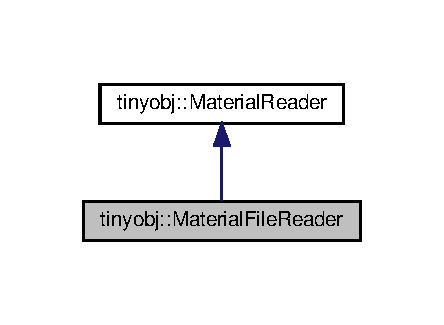
\includegraphics[width=213pt]{classtinyobj_1_1MaterialFileReader__inherit__graph}
\end{center}
\end{figure}


Collaboration diagram for tinyobj\+:\+:Material\+File\+Reader\+:\nopagebreak
\begin{figure}[H]
\begin{center}
\leavevmode
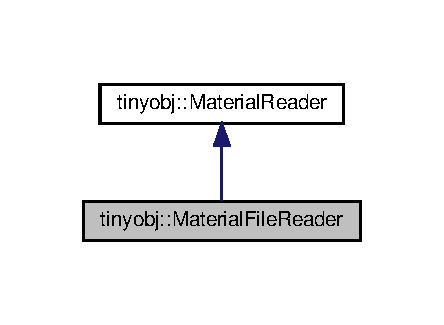
\includegraphics[width=213pt]{classtinyobj_1_1MaterialFileReader__coll__graph}
\end{center}
\end{figure}
\subsection*{Public Member Functions}
\begin{DoxyCompactItemize}
\item 
\mbox{\Hypertarget{classtinyobj_1_1MaterialFileReader_a824d0100284310fe213d86ad443cc575}\label{classtinyobj_1_1MaterialFileReader_a824d0100284310fe213d86ad443cc575}} 
{\bfseries Material\+File\+Reader} (const std\+::string \&mtl\+\_\+basepath)
\item 
\mbox{\Hypertarget{classtinyobj_1_1MaterialFileReader_a9374212c9997aa8ac0d15d97f67b25f8}\label{classtinyobj_1_1MaterialFileReader_a9374212c9997aa8ac0d15d97f67b25f8}} 
virtual std\+::string {\bfseries operator()} (const std\+::string \&mat\+Id, std\+::vector$<$ \hyperlink{structtinyobj_1_1material__t}{material\+\_\+t} $>$ \&materials, std\+::map$<$ std\+::string, int $>$ \&mat\+Map)
\end{DoxyCompactItemize}


The documentation for this class was generated from the following files\+:\begin{DoxyCompactItemize}
\item 
/media/msgro/\+Maxtor/\+World\+\_\+\+Imaker/\+World\+\_\+\+Imaker\+\_\+merge/\+World\+\_\+\+Imaker/glimac/src/tiny\+\_\+obj\+\_\+loader.\+h\item 
/media/msgro/\+Maxtor/\+World\+\_\+\+Imaker/\+World\+\_\+\+Imaker\+\_\+merge/\+World\+\_\+\+Imaker/glimac/src/tiny\+\_\+obj\+\_\+loader.\+cpp\end{DoxyCompactItemize}

\hypertarget{classtinyobj_1_1MaterialReader}{}\section{tinyobj\+:\+:Material\+Reader Class Reference}
\label{classtinyobj_1_1MaterialReader}\index{tinyobj\+::\+Material\+Reader@{tinyobj\+::\+Material\+Reader}}


Inheritance diagram for tinyobj\+:\+:Material\+Reader\+:\nopagebreak
\begin{figure}[H]
\begin{center}
\leavevmode
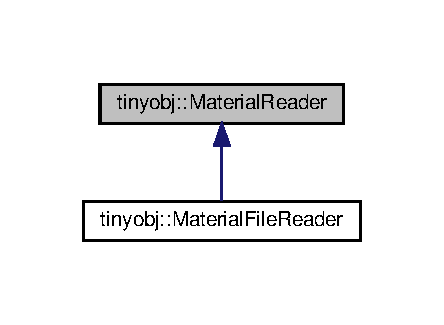
\includegraphics[width=213pt]{classtinyobj_1_1MaterialReader__inherit__graph}
\end{center}
\end{figure}
\subsection*{Public Member Functions}
\begin{DoxyCompactItemize}
\item 
\mbox{\Hypertarget{classtinyobj_1_1MaterialReader_afc27ac917abd33dc3ec4a9ae7a519962}\label{classtinyobj_1_1MaterialReader_afc27ac917abd33dc3ec4a9ae7a519962}} 
virtual std\+::string {\bfseries operator()} (const std\+::string \&mat\+Id, std\+::vector$<$ \hyperlink{structtinyobj_1_1material__t}{material\+\_\+t} $>$ \&materials, std\+::map$<$ std\+::string, int $>$ \&mat\+Map)=0
\end{DoxyCompactItemize}


The documentation for this class was generated from the following file\+:\begin{DoxyCompactItemize}
\item 
/home/6im2/amansion/\+Documents/\+P\+R\+O\+J\+E\+T/\+World\+\_\+\+Imaker/glimac/src/tiny\+\_\+obj\+\_\+loader.\+h\end{DoxyCompactItemize}

\hypertarget{structtinyobj_1_1mesh__t}{}\section{tinyobj\+:\+:mesh\+\_\+t Struct Reference}
\label{structtinyobj_1_1mesh__t}\index{tinyobj\+::mesh\+\_\+t@{tinyobj\+::mesh\+\_\+t}}
\subsection*{Public Attributes}
\begin{DoxyCompactItemize}
\item 
\mbox{\Hypertarget{structtinyobj_1_1mesh__t_a3014a27913256384aa283345b69ff2ec}\label{structtinyobj_1_1mesh__t_a3014a27913256384aa283345b69ff2ec}} 
std\+::vector$<$ float $>$ {\bfseries positions}
\item 
\mbox{\Hypertarget{structtinyobj_1_1mesh__t_a28c2f7eb3114e6ed82a5b7326a4e7a1c}\label{structtinyobj_1_1mesh__t_a28c2f7eb3114e6ed82a5b7326a4e7a1c}} 
std\+::vector$<$ float $>$ {\bfseries normals}
\item 
\mbox{\Hypertarget{structtinyobj_1_1mesh__t_a0fc485afc76bcd7e147b22285d7d6575}\label{structtinyobj_1_1mesh__t_a0fc485afc76bcd7e147b22285d7d6575}} 
std\+::vector$<$ float $>$ {\bfseries texcoords}
\item 
\mbox{\Hypertarget{structtinyobj_1_1mesh__t_aa0a07f40559a650e6917c506d78e298a}\label{structtinyobj_1_1mesh__t_aa0a07f40559a650e6917c506d78e298a}} 
std\+::vector$<$ unsigned int $>$ {\bfseries indices}
\item 
\mbox{\Hypertarget{structtinyobj_1_1mesh__t_a57b2f12dfa3fd620b25babcd3a09ec6b}\label{structtinyobj_1_1mesh__t_a57b2f12dfa3fd620b25babcd3a09ec6b}} 
std\+::vector$<$ int $>$ {\bfseries material\+\_\+ids}
\end{DoxyCompactItemize}


The documentation for this struct was generated from the following file\+:\begin{DoxyCompactItemize}
\item 
/home/6im2/amansion/\+Documents/\+P\+R\+O\+J\+E\+T/\+World\+\_\+\+Imaker/glimac/src/tiny\+\_\+obj\+\_\+loader.\+h\end{DoxyCompactItemize}

\hypertarget{structtinyobj_1_1obj__shape}{}\section{tinyobj\+:\+:obj\+\_\+shape Struct Reference}
\label{structtinyobj_1_1obj__shape}\index{tinyobj\+::obj\+\_\+shape@{tinyobj\+::obj\+\_\+shape}}
\subsection*{Public Attributes}
\begin{DoxyCompactItemize}
\item 
\mbox{\Hypertarget{structtinyobj_1_1obj__shape_ad088c2525809a91953fca51798f64b89}\label{structtinyobj_1_1obj__shape_ad088c2525809a91953fca51798f64b89}} 
std\+::vector$<$ float $>$ {\bfseries v}
\item 
\mbox{\Hypertarget{structtinyobj_1_1obj__shape_ac87ced8cdff16da62a202bd390e77a8e}\label{structtinyobj_1_1obj__shape_ac87ced8cdff16da62a202bd390e77a8e}} 
std\+::vector$<$ float $>$ {\bfseries vn}
\item 
\mbox{\Hypertarget{structtinyobj_1_1obj__shape_a2d6dcc97e66ca2596dd50236c899b456}\label{structtinyobj_1_1obj__shape_a2d6dcc97e66ca2596dd50236c899b456}} 
std\+::vector$<$ float $>$ {\bfseries vt}
\end{DoxyCompactItemize}


The documentation for this struct was generated from the following file\+:\begin{DoxyCompactItemize}
\item 
/media/msgro/\+Maxtor/\+World\+\_\+\+Imaker/\+World\+\_\+\+Imaker/glimac/src/tiny\+\_\+obj\+\_\+loader.\+cpp\end{DoxyCompactItemize}

\hypertarget{classglimac_1_1Program}{}\section{glimac\+:\+:Program Class Reference}
\label{classglimac_1_1Program}\index{glimac\+::\+Program@{glimac\+::\+Program}}
\subsection*{Public Member Functions}
\begin{DoxyCompactItemize}
\item 
\mbox{\Hypertarget{classglimac_1_1Program_aad59ed1f53824eda09b95fd1acdce674}\label{classglimac_1_1Program_aad59ed1f53824eda09b95fd1acdce674}} 
{\bfseries Program} (\hyperlink{classglimac_1_1Program}{Program} \&\&rvalue)
\item 
\mbox{\Hypertarget{classglimac_1_1Program_a3ee1eac00a2e3fa4b6bab51d4333f33c}\label{classglimac_1_1Program_a3ee1eac00a2e3fa4b6bab51d4333f33c}} 
\hyperlink{classglimac_1_1Program}{Program} \& {\bfseries operator=} (\hyperlink{classglimac_1_1Program}{Program} \&\&rvalue)
\item 
\mbox{\Hypertarget{classglimac_1_1Program_ab1a519d005c77ba44876d1f309b38d18}\label{classglimac_1_1Program_ab1a519d005c77ba44876d1f309b38d18}} 
G\+Luint {\bfseries get\+G\+L\+Id} () const
\item 
\mbox{\Hypertarget{classglimac_1_1Program_a5aac165d28cd6f704c01a3e0eee2119d}\label{classglimac_1_1Program_a5aac165d28cd6f704c01a3e0eee2119d}} 
void {\bfseries attach\+Shader} (const \hyperlink{classglimac_1_1Shader}{Shader} \&shader)
\item 
\mbox{\Hypertarget{classglimac_1_1Program_a2f32f4f66ff9742750418f6fda054931}\label{classglimac_1_1Program_a2f32f4f66ff9742750418f6fda054931}} 
bool {\bfseries link} ()
\item 
\mbox{\Hypertarget{classglimac_1_1Program_aaf1769457ca41bca4afad7ecf90e9c3f}\label{classglimac_1_1Program_aaf1769457ca41bca4afad7ecf90e9c3f}} 
const std\+::string {\bfseries get\+Info\+Log} () const
\item 
\mbox{\Hypertarget{classglimac_1_1Program_a825cb4d58cccdf849730191ae5e118c6}\label{classglimac_1_1Program_a825cb4d58cccdf849730191ae5e118c6}} 
void {\bfseries use} () const
\end{DoxyCompactItemize}


The documentation for this class was generated from the following files\+:\begin{DoxyCompactItemize}
\item 
/media/msgro/\+Maxtor/\+World\+\_\+\+Imaker/\+World\+\_\+\+Imaker\+\_\+merge/\+World\+\_\+\+Imaker/glimac/include/glimac/\hyperlink{Program_8hpp}{Program.\+hpp}\item 
/media/msgro/\+Maxtor/\+World\+\_\+\+Imaker/\+World\+\_\+\+Imaker\+\_\+merge/\+World\+\_\+\+Imaker/glimac/src/\hyperlink{Program_8cpp}{Program.\+cpp}\end{DoxyCompactItemize}

\hypertarget{classglimac_1_1SDLWindowManager}{}\section{glimac\+:\+:S\+D\+L\+Window\+Manager Class Reference}
\label{classglimac_1_1SDLWindowManager}\index{glimac\+::\+S\+D\+L\+Window\+Manager@{glimac\+::\+S\+D\+L\+Window\+Manager}}
\subsection*{Public Member Functions}
\begin{DoxyCompactItemize}
\item 
\mbox{\Hypertarget{classglimac_1_1SDLWindowManager_aaddb3bc2ec58bc1e818276e81605520f}\label{classglimac_1_1SDLWindowManager_aaddb3bc2ec58bc1e818276e81605520f}} 
{\bfseries S\+D\+L\+Window\+Manager} (uint32\+\_\+t width, uint32\+\_\+t height, const char $\ast$title)
\item 
\mbox{\Hypertarget{classglimac_1_1SDLWindowManager_a4b2fd3e74f00c28d3b03e0cff3bb0131}\label{classglimac_1_1SDLWindowManager_a4b2fd3e74f00c28d3b03e0cff3bb0131}} 
bool {\bfseries poll\+Event} (S\+D\+L\+\_\+\+Event \&e)
\item 
\mbox{\Hypertarget{classglimac_1_1SDLWindowManager_aa5941f14a1a2098da1a072b2dac43930}\label{classglimac_1_1SDLWindowManager_aa5941f14a1a2098da1a072b2dac43930}} 
bool {\bfseries is\+Key\+Pressed} (S\+D\+L\+\_\+\+Keycode key) const
\item 
\mbox{\Hypertarget{classglimac_1_1SDLWindowManager_a3f970279f069c97d64845687f1af5743}\label{classglimac_1_1SDLWindowManager_a3f970279f069c97d64845687f1af5743}} 
bool {\bfseries is\+Mouse\+Button\+Pressed} (uint32\+\_\+t button) const
\item 
\mbox{\Hypertarget{classglimac_1_1SDLWindowManager_aac32964a8c7e0e0e790b8fab29ac2831}\label{classglimac_1_1SDLWindowManager_aac32964a8c7e0e0e790b8fab29ac2831}} 
glm\+::ivec2 {\bfseries get\+Mouse\+Position} () const
\item 
\mbox{\Hypertarget{classglimac_1_1SDLWindowManager_aee6b4f60e5b418a99d35360aea48bd41}\label{classglimac_1_1SDLWindowManager_aee6b4f60e5b418a99d35360aea48bd41}} 
void {\bfseries swap\+Buffers} ()
\item 
\mbox{\Hypertarget{classglimac_1_1SDLWindowManager_ae79e8321234999083adda1287cf825fe}\label{classglimac_1_1SDLWindowManager_ae79e8321234999083adda1287cf825fe}} 
float {\bfseries get\+Time} () const
\item 
\mbox{\Hypertarget{classglimac_1_1SDLWindowManager_ae4ddac1da16f866bbd2bd685556afe8e}\label{classglimac_1_1SDLWindowManager_ae4ddac1da16f866bbd2bd685556afe8e}} 
void {\bfseries print\+Signature} ()
\end{DoxyCompactItemize}
\subsection*{Public Attributes}
\begin{DoxyCompactItemize}
\item 
\mbox{\Hypertarget{classglimac_1_1SDLWindowManager_a5999492fdc73a660c624015485a8a71e}\label{classglimac_1_1SDLWindowManager_a5999492fdc73a660c624015485a8a71e}} 
S\+D\+L\+\_\+\+Window $\ast$ {\bfseries window}
\end{DoxyCompactItemize}


The documentation for this class was generated from the following files\+:\begin{DoxyCompactItemize}
\item 
/home/6im2/amansion/\+Documents/\+P\+R\+O\+J\+E\+T/\+World\+\_\+\+Imaker/glimac/include/glimac/\hyperlink{SDLWindowManager_8hpp}{S\+D\+L\+Window\+Manager.\+hpp}\item 
/home/6im2/amansion/\+Documents/\+P\+R\+O\+J\+E\+T/\+World\+\_\+\+Imaker/glimac/src/\hyperlink{SDLWindowManager_8cpp}{S\+D\+L\+Window\+Manager.\+cpp}\end{DoxyCompactItemize}

\hypertarget{classglimac_1_1Shader}{}\section{glimac\+:\+:Shader Class Reference}
\label{classglimac_1_1Shader}\index{glimac\+::\+Shader@{glimac\+::\+Shader}}
\subsection*{Public Member Functions}
\begin{DoxyCompactItemize}
\item 
\mbox{\Hypertarget{classglimac_1_1Shader_a064a1d24851c1c405d3c912cff9521c4}\label{classglimac_1_1Shader_a064a1d24851c1c405d3c912cff9521c4}} 
{\bfseries Shader} (G\+Lenum type)
\item 
\mbox{\Hypertarget{classglimac_1_1Shader_a98bf794b782f89a7a5c859607e6dc62b}\label{classglimac_1_1Shader_a98bf794b782f89a7a5c859607e6dc62b}} 
{\bfseries Shader} (\hyperlink{classglimac_1_1Shader}{Shader} \&\&rvalue)
\item 
\mbox{\Hypertarget{classglimac_1_1Shader_a0790eeb7a9fc154161bee6b78e287828}\label{classglimac_1_1Shader_a0790eeb7a9fc154161bee6b78e287828}} 
\hyperlink{classglimac_1_1Shader}{Shader} \& {\bfseries operator=} (\hyperlink{classglimac_1_1Shader}{Shader} \&\&rvalue)
\item 
\mbox{\Hypertarget{classglimac_1_1Shader_a46c21c4b6b9ee89426b458695897202e}\label{classglimac_1_1Shader_a46c21c4b6b9ee89426b458695897202e}} 
G\+Luint {\bfseries get\+G\+L\+Id} () const
\item 
\mbox{\Hypertarget{classglimac_1_1Shader_a66701118e7f1d789a258936c82b32874}\label{classglimac_1_1Shader_a66701118e7f1d789a258936c82b32874}} 
void {\bfseries set\+Source} (const char $\ast$src)
\item 
\mbox{\Hypertarget{classglimac_1_1Shader_a1e6c6814a6275dd698b3befdb89aa647}\label{classglimac_1_1Shader_a1e6c6814a6275dd698b3befdb89aa647}} 
bool {\bfseries compile} ()
\item 
\mbox{\Hypertarget{classglimac_1_1Shader_aa0de6702041087187d8eca874000cfa6}\label{classglimac_1_1Shader_aa0de6702041087187d8eca874000cfa6}} 
const std\+::string {\bfseries get\+Info\+Log} () const
\end{DoxyCompactItemize}


The documentation for this class was generated from the following files\+:\begin{DoxyCompactItemize}
\item 
/media/msgro/\+Maxtor/\+World\+\_\+\+Imaker/\+World\+\_\+\+Imaker/glimac/include/glimac/Shader.\+hpp\item 
/media/msgro/\+Maxtor/\+World\+\_\+\+Imaker/\+World\+\_\+\+Imaker/glimac/src/Shader.\+cpp\end{DoxyCompactItemize}

\hypertarget{structtinyobj_1_1shape__t}{}\section{tinyobj\+:\+:shape\+\_\+t Struct Reference}
\label{structtinyobj_1_1shape__t}\index{tinyobj\+::shape\+\_\+t@{tinyobj\+::shape\+\_\+t}}


Collaboration diagram for tinyobj\+:\+:shape\+\_\+t\+:
\nopagebreak
\begin{figure}[H]
\begin{center}
\leavevmode
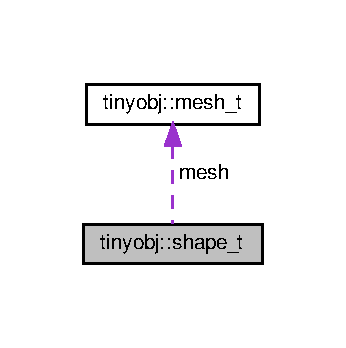
\includegraphics[width=166pt]{structtinyobj_1_1shape__t__coll__graph}
\end{center}
\end{figure}
\subsection*{Public Attributes}
\begin{DoxyCompactItemize}
\item 
\mbox{\Hypertarget{structtinyobj_1_1shape__t_a98650e2e66d00934f68de88eafb34630}\label{structtinyobj_1_1shape__t_a98650e2e66d00934f68de88eafb34630}} 
std\+::string {\bfseries name}
\item 
\mbox{\Hypertarget{structtinyobj_1_1shape__t_a3dacb06dfbfe9e245ff4bc7b5b3d9818}\label{structtinyobj_1_1shape__t_a3dacb06dfbfe9e245ff4bc7b5b3d9818}} 
\hyperlink{structtinyobj_1_1mesh__t}{mesh\+\_\+t} {\bfseries mesh}
\end{DoxyCompactItemize}


The documentation for this struct was generated from the following file\+:\begin{DoxyCompactItemize}
\item 
/media/msgro/\+Maxtor/\+World\+\_\+\+Imaker/\+World\+\_\+\+Imaker\+\_\+merge/\+World\+\_\+\+Imaker/glimac/src/tiny\+\_\+obj\+\_\+loader.\+h\end{DoxyCompactItemize}

\hypertarget{structglimac_1_1ShapeVertex}{}\section{glimac\+:\+:Shape\+Vertex Struct Reference}
\label{structglimac_1_1ShapeVertex}\index{glimac\+::\+Shape\+Vertex@{glimac\+::\+Shape\+Vertex}}
\subsection*{Public Attributes}
\begin{DoxyCompactItemize}
\item 
\mbox{\Hypertarget{structglimac_1_1ShapeVertex_a727bc4adace4f00e47069ce7373e3b97}\label{structglimac_1_1ShapeVertex_a727bc4adace4f00e47069ce7373e3b97}} 
glm\+::vec3 {\bfseries position}
\item 
\mbox{\Hypertarget{structglimac_1_1ShapeVertex_af8ef5c93da6bc86b5dcfa3d8e2a8fc21}\label{structglimac_1_1ShapeVertex_af8ef5c93da6bc86b5dcfa3d8e2a8fc21}} 
glm\+::vec3 {\bfseries normal}
\item 
\mbox{\Hypertarget{structglimac_1_1ShapeVertex_ab694e76716c4cdc5e8636325b5fbeee2}\label{structglimac_1_1ShapeVertex_ab694e76716c4cdc5e8636325b5fbeee2}} 
glm\+::vec2 {\bfseries tex\+Coords}
\end{DoxyCompactItemize}


The documentation for this struct was generated from the following file\+:\begin{DoxyCompactItemize}
\item 
/home/6im2/amansion/\+Documents/\+P\+R\+O\+J\+E\+T/\+World\+\_\+\+Imaker/glimac/include/glimac/common.\+hpp\end{DoxyCompactItemize}

\hypertarget{structstbi__io__callbacks}{}\section{stbi\+\_\+io\+\_\+callbacks Struct Reference}
\label{structstbi__io__callbacks}\index{stbi\+\_\+io\+\_\+callbacks@{stbi\+\_\+io\+\_\+callbacks}}
\subsection*{Public Attributes}
\begin{DoxyCompactItemize}
\item 
\mbox{\Hypertarget{structstbi__io__callbacks_a623e46b3a2a019611601409926283a88}\label{structstbi__io__callbacks_a623e46b3a2a019611601409926283a88}} 
int($\ast$ {\bfseries read} )(void $\ast$user, char $\ast$data, int size)
\item 
\mbox{\Hypertarget{structstbi__io__callbacks_a257aac5480a90a6c4b8fbe86c1b01068}\label{structstbi__io__callbacks_a257aac5480a90a6c4b8fbe86c1b01068}} 
void($\ast$ {\bfseries skip} )(void $\ast$user, int n)
\item 
\mbox{\Hypertarget{structstbi__io__callbacks_a319639db2f76e715eed7a7a974136832}\label{structstbi__io__callbacks_a319639db2f76e715eed7a7a974136832}} 
int($\ast$ {\bfseries eof} )(void $\ast$user)
\end{DoxyCompactItemize}


The documentation for this struct was generated from the following file\+:\begin{DoxyCompactItemize}
\item 
/home/6im2/amansion/\+Documents/\+P\+R\+O\+J\+E\+T/\+World\+\_\+\+Imaker/glimac/include/glimac/stb\+\_\+image.\+h\end{DoxyCompactItemize}

\hypertarget{classglimac_1_1Texture}{}\section{glimac\+:\+:Texture Class Reference}
\label{classglimac_1_1Texture}\index{glimac\+::\+Texture@{glimac\+::\+Texture}}
\subsection*{Public Member Functions}
\begin{DoxyCompactItemize}
\item 
\mbox{\Hypertarget{classglimac_1_1Texture_a2a1e06217a8c98f4ddd7c271b7590c03}\label{classglimac_1_1Texture_a2a1e06217a8c98f4ddd7c271b7590c03}} 
void {\bfseries set\+Uniform\+Location} (\hyperlink{classglimac_1_1Program}{Program} \&program, const G\+Lchar $\ast$name)
\item 
\mbox{\Hypertarget{classglimac_1_1Texture_a412726a887d5b80d6382e0d25584661f}\label{classglimac_1_1Texture_a412726a887d5b80d6382e0d25584661f}} 
void {\bfseries set\+Image} (const \hyperlink{classglimac_1_1FilePath}{File\+Path} \&filepath)
\item 
\mbox{\Hypertarget{classglimac_1_1Texture_aab4d5370b02499884260a3ce9e7349be}\label{classglimac_1_1Texture_aab4d5370b02499884260a3ce9e7349be}} 
G\+Luint {\bfseries get\+Texture} ()
\item 
\mbox{\Hypertarget{classglimac_1_1Texture_ac222b4e2c040a8b64484bb60eb73574f}\label{classglimac_1_1Texture_ac222b4e2c040a8b64484bb60eb73574f}} 
G\+Luint $\ast$ {\bfseries get\+Texture\+Pointer} ()
\item 
\mbox{\Hypertarget{classglimac_1_1Texture_af27c9e6a54fe8a60cedaad97d8acbcae}\label{classglimac_1_1Texture_af27c9e6a54fe8a60cedaad97d8acbcae}} 
unsigned int {\bfseries get\+Image\+Width} ()
\item 
\mbox{\Hypertarget{classglimac_1_1Texture_a66760a2dc586c0780ee3b9961048424b}\label{classglimac_1_1Texture_a66760a2dc586c0780ee3b9961048424b}} 
unsigned int {\bfseries get\+Image\+Height} ()
\item 
\mbox{\Hypertarget{classglimac_1_1Texture_a7060818013d2bfbe42df5d0b01f2825d}\label{classglimac_1_1Texture_a7060818013d2bfbe42df5d0b01f2825d}} 
const glm\+::vec4 $\ast$ {\bfseries get\+Image\+Pixels} () const
\item 
\mbox{\Hypertarget{classglimac_1_1Texture_a80d018b2208095d54c3439e6328761ff}\label{classglimac_1_1Texture_a80d018b2208095d54c3439e6328761ff}} 
G\+Luint {\bfseries get\+Uniform\+Location} ()
\end{DoxyCompactItemize}


The documentation for this class was generated from the following files\+:\begin{DoxyCompactItemize}
\item 
/media/msgro/\+Maxtor/\+World\+\_\+\+Imaker/\+World\+\_\+\+Imaker\+\_\+merge/\+World\+\_\+\+Imaker/glimac/include/glimac/Texture.\+hpp\item 
/media/msgro/\+Maxtor/\+World\+\_\+\+Imaker/\+World\+\_\+\+Imaker\+\_\+merge/\+World\+\_\+\+Imaker/glimac/src/Texture.\+cpp\end{DoxyCompactItemize}

\hypertarget{structglimac_1_1Vertex3DTexture}{}\section{glimac\+:\+:Vertex3\+D\+Texture Struct Reference}
\label{structglimac_1_1Vertex3DTexture}\index{glimac\+::\+Vertex3\+D\+Texture@{glimac\+::\+Vertex3\+D\+Texture}}
\subsection*{Public Member Functions}
\begin{DoxyCompactItemize}
\item 
\mbox{\Hypertarget{structglimac_1_1Vertex3DTexture_ac461f0825c04dd162e732cdcf61bce8b}\label{structglimac_1_1Vertex3DTexture_ac461f0825c04dd162e732cdcf61bce8b}} 
{\bfseries Vertex3\+D\+Texture} (glm\+::vec3 position, glm\+::vec3 normal, glm\+::vec2 texture)
\end{DoxyCompactItemize}
\subsection*{Public Attributes}
\begin{DoxyCompactItemize}
\item 
\mbox{\Hypertarget{structglimac_1_1Vertex3DTexture_ac14c3d140276a6e99414c73c10f501b5}\label{structglimac_1_1Vertex3DTexture_ac14c3d140276a6e99414c73c10f501b5}} 
glm\+::vec3 {\bfseries position}
\item 
\mbox{\Hypertarget{structglimac_1_1Vertex3DTexture_af96395447e991b64d3871618b60b7e41}\label{structglimac_1_1Vertex3DTexture_af96395447e991b64d3871618b60b7e41}} 
glm\+::vec3 {\bfseries normal}
\item 
\mbox{\Hypertarget{structglimac_1_1Vertex3DTexture_a7dc16eb566e2fb5cac456f001449faa0}\label{structglimac_1_1Vertex3DTexture_a7dc16eb566e2fb5cac456f001449faa0}} 
glm\+::vec2 {\bfseries texture}
\end{DoxyCompactItemize}


The documentation for this struct was generated from the following file\+:\begin{DoxyCompactItemize}
\item 
/media/msgro/\+Maxtor/\+World\+\_\+\+Imaker/\+World\+\_\+\+Imaker/glimac/include/glimac/common.\+hpp\end{DoxyCompactItemize}

\hypertarget{structtinyobj_1_1vertex__index}{}\section{tinyobj\+:\+:vertex\+\_\+index Struct Reference}
\label{structtinyobj_1_1vertex__index}\index{tinyobj\+::vertex\+\_\+index@{tinyobj\+::vertex\+\_\+index}}
\subsection*{Public Member Functions}
\begin{DoxyCompactItemize}
\item 
\mbox{\Hypertarget{structtinyobj_1_1vertex__index_a894075fa64d32082219c138f111e4753}\label{structtinyobj_1_1vertex__index_a894075fa64d32082219c138f111e4753}} 
{\bfseries vertex\+\_\+index} (int idx)
\item 
\mbox{\Hypertarget{structtinyobj_1_1vertex__index_aa3c4d6bcba36c2abb06e25497a1376a1}\label{structtinyobj_1_1vertex__index_aa3c4d6bcba36c2abb06e25497a1376a1}} 
{\bfseries vertex\+\_\+index} (int vidx, int vtidx, int vnidx)
\end{DoxyCompactItemize}
\subsection*{Public Attributes}
\begin{DoxyCompactItemize}
\item 
\mbox{\Hypertarget{structtinyobj_1_1vertex__index_a91a2616fb97e0da915a40654edf9b558}\label{structtinyobj_1_1vertex__index_a91a2616fb97e0da915a40654edf9b558}} 
int {\bfseries v\+\_\+idx}
\item 
\mbox{\Hypertarget{structtinyobj_1_1vertex__index_aae7e058d3aa0993aa05e95d82dd6b8bf}\label{structtinyobj_1_1vertex__index_aae7e058d3aa0993aa05e95d82dd6b8bf}} 
int {\bfseries vt\+\_\+idx}
\item 
\mbox{\Hypertarget{structtinyobj_1_1vertex__index_a30f2a63a5ed20cc3ad64e340c4020da8}\label{structtinyobj_1_1vertex__index_a30f2a63a5ed20cc3ad64e340c4020da8}} 
int {\bfseries vn\+\_\+idx}
\end{DoxyCompactItemize}


The documentation for this struct was generated from the following file\+:\begin{DoxyCompactItemize}
\item 
/home/6im2/amansion/\+Documents/\+P\+R\+O\+J\+E\+T/\+World\+\_\+\+Imaker/glimac/src/tiny\+\_\+obj\+\_\+loader.\+cpp\end{DoxyCompactItemize}

\chapter{File Documentation}
\hypertarget{Cube_8hpp}{}\section{/media/msgro/\+Maxtor/\+World\+\_\+\+Imaker/\+World\+\_\+\+Imaker\+\_\+merge/\+World\+\_\+\+Imaker/glimac/include/glimac/\+Cube.hpp File Reference}
\label{Cube_8hpp}\index{/media/msgro/\+Maxtor/\+World\+\_\+\+Imaker/\+World\+\_\+\+Imaker\+\_\+merge/\+World\+\_\+\+Imaker/glimac/include/glimac/\+Cube.\+hpp@{/media/msgro/\+Maxtor/\+World\+\_\+\+Imaker/\+World\+\_\+\+Imaker\+\_\+merge/\+World\+\_\+\+Imaker/glimac/include/glimac/\+Cube.\+hpp}}


Gestion des cubes.  


{\ttfamily \#include \char`\"{}common.\+hpp\char`\"{}}\newline
Include dependency graph for Cube.\+hpp\+:
\nopagebreak
\begin{figure}[H]
\begin{center}
\leavevmode
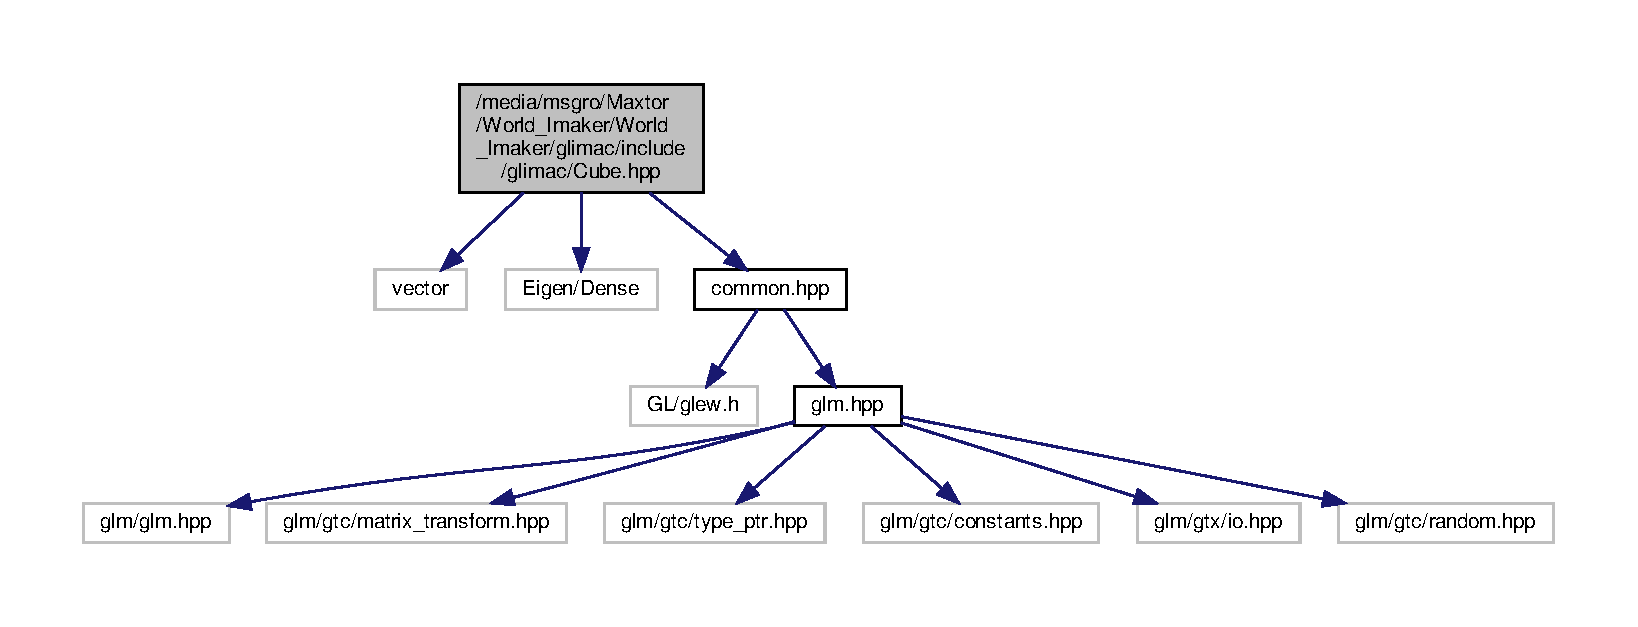
\includegraphics[width=350pt]{Cube_8hpp__incl}
\end{center}
\end{figure}
This graph shows which files directly or indirectly include this file\+:
\nopagebreak
\begin{figure}[H]
\begin{center}
\leavevmode
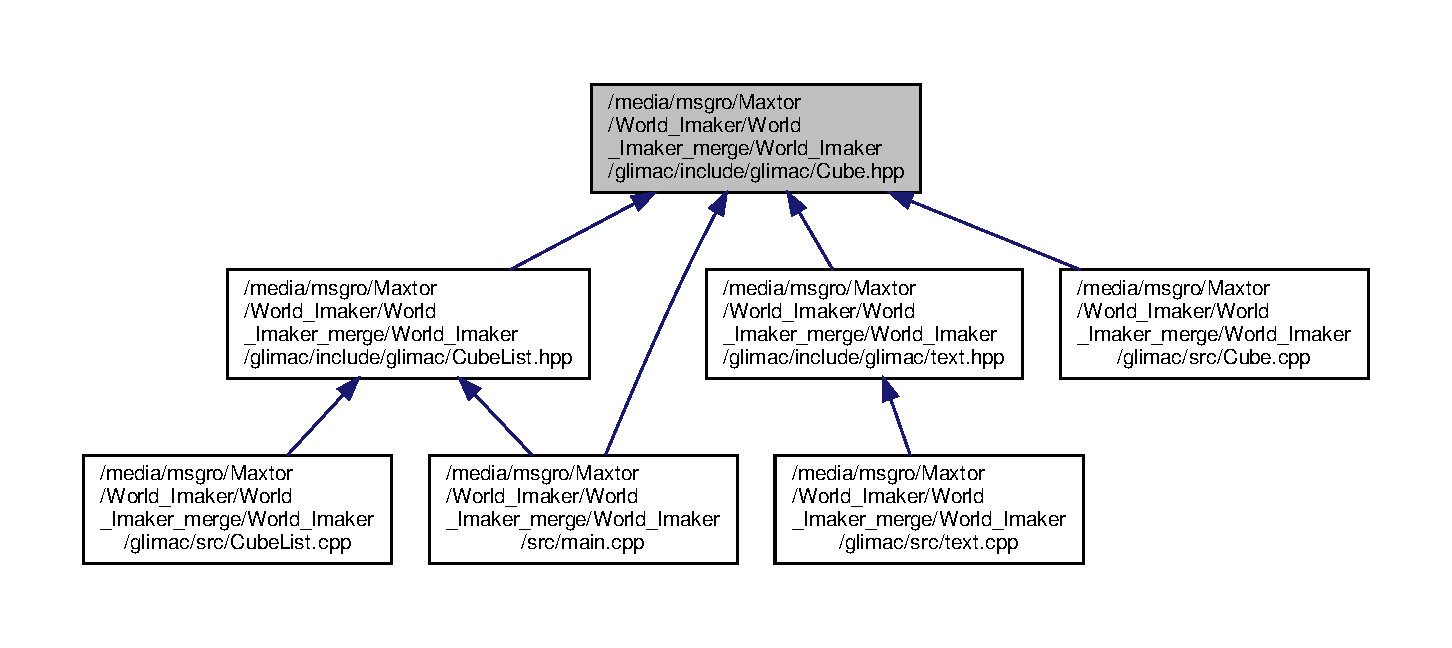
\includegraphics[width=350pt]{Cube_8hpp__dep__incl}
\end{center}
\end{figure}
\subsection*{Classes}
\begin{DoxyCompactItemize}
\item 
class \hyperlink{classglimac_1_1Cube}{glimac\+::\+Cube}
\begin{DoxyCompactList}\small\item\em Classe representant un cube. \end{DoxyCompactList}\end{DoxyCompactItemize}
\subsection*{Namespaces}
\begin{DoxyCompactItemize}
\item 
 \hyperlink{namespaceglimac}{glimac}
\begin{DoxyCompactList}\small\item\em Outils de gestion d\textquotesingle{}une scène 3D. \end{DoxyCompactList}\end{DoxyCompactItemize}


\subsection{Detailed Description}
Gestion des cubes. 

\begin{DoxyAuthor}{Author}
M\+A\+N\+S\+I\+ON Amélia \& S\+G\+RO\textquotesingle{} Manon 
\end{DoxyAuthor}
\begin{DoxyVersion}{Version}
0.\+1 
\end{DoxyVersion}
\begin{DoxyDate}{Date}
20 décembre 2019
\end{DoxyDate}
Gestion des cubes dans la scène (sur les axes x,y,z) 
\hypertarget{main_8cpp}{}\section{/media/msgro/\+Maxtor/\+World\+\_\+\+Imaker/\+World\+\_\+\+Imaker\+\_\+merge/\+World\+\_\+\+Imaker/src/main.cpp File Reference}
\label{main_8cpp}\index{/media/msgro/\+Maxtor/\+World\+\_\+\+Imaker/\+World\+\_\+\+Imaker\+\_\+merge/\+World\+\_\+\+Imaker/src/main.\+cpp@{/media/msgro/\+Maxtor/\+World\+\_\+\+Imaker/\+World\+\_\+\+Imaker\+\_\+merge/\+World\+\_\+\+Imaker/src/main.\+cpp}}


Programme principal -\/ Editeur de scène 3D.  


{\ttfamily \#include $<$G\+L/glew.\+h$>$}\newline
{\ttfamily \#include $<$iostream$>$}\newline
{\ttfamily \#include $<$fstream$>$}\newline
{\ttfamily \#include $<$string$>$}\newline
{\ttfamily \#include $<$cstring$>$}\newline
{\ttfamily \#include $<$cstddef$>$}\newline
{\ttfamily \#include $<$vector$>$}\newline
{\ttfamily \#include $<$stack$>$}\newline
{\ttfamily \#include $<$stdio.\+h$>$}\newline
{\ttfamily \#include $<$stdlib.\+h$>$}\newline
{\ttfamily \#include $<$glm/glm.\+hpp$>$}\newline
{\ttfamily \#include $<$glimac/\+S\+D\+L\+Window\+Manager.\+hpp$>$}\newline
{\ttfamily \#include $<$glimac/\+Program.\+hpp$>$}\newline
{\ttfamily \#include $<$glimac/\+File\+Path.\+hpp$>$}\newline
{\ttfamily \#include $<$glimac/glm.\+hpp$>$}\newline
{\ttfamily \#include $<$glimac/\+Image.\+hpp$>$}\newline
{\ttfamily \#include $<$glimac/\+Cube.\+hpp$>$}\newline
{\ttfamily \#include $<$glimac/\+Texture.\+hpp$>$}\newline
{\ttfamily \#include $<$glimac/\+Cube\+List.\+hpp$>$}\newline
{\ttfamily \#include $<$glimac/\+Controls.\+hpp$>$}\newline
{\ttfamily \#include $<$include/imgui.\+h$>$}\newline
{\ttfamily \#include $<$examples/imgui\+\_\+impl\+\_\+sdl.\+h$>$}\newline
{\ttfamily \#include $<$examples/imgui\+\_\+impl\+\_\+opengl3.\+h$>$}\newline
{\ttfamily \#include $<$misc/cpp/imgui\+\_\+stdlib.\+h$>$}\newline
Include dependency graph for main.\+cpp\+:
\nopagebreak
\begin{figure}[H]
\begin{center}
\leavevmode
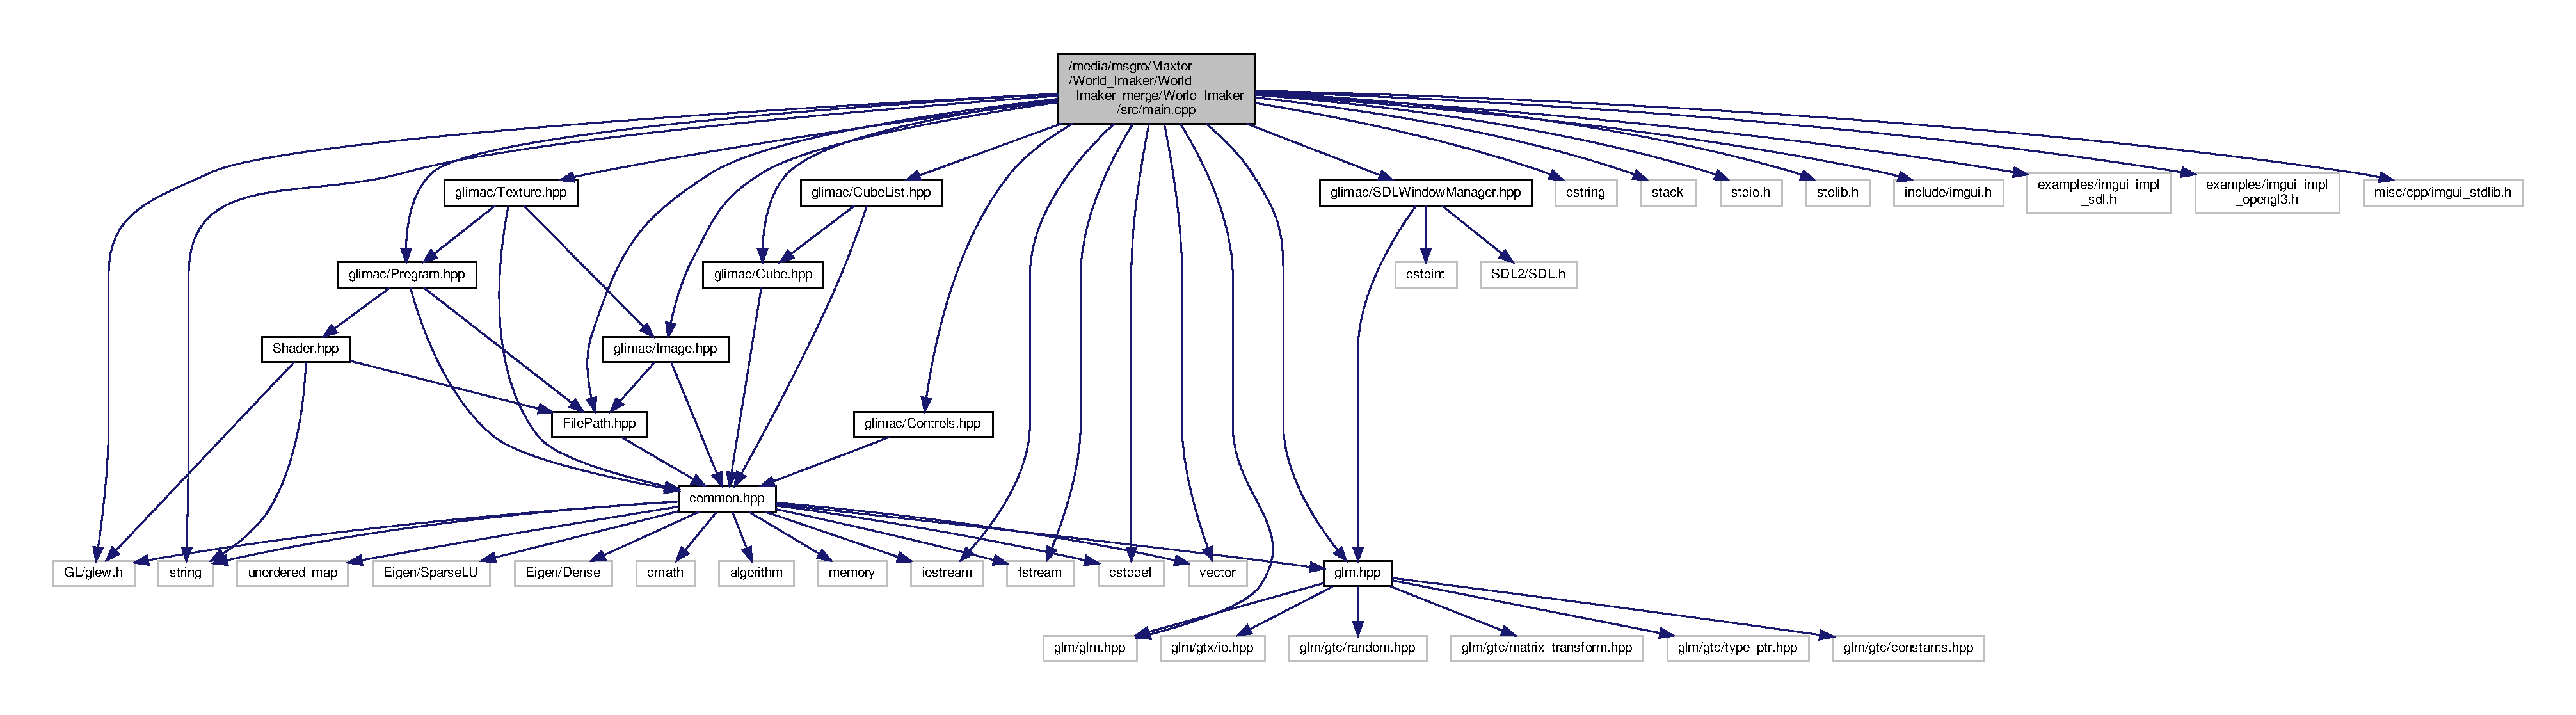
\includegraphics[width=350pt]{main_8cpp__incl}
\end{center}
\end{figure}
\subsection*{Functions}
\begin{DoxyCompactItemize}
\item 
int \hyperlink{main_8cpp_a3c04138a5bfe5d72780bb7e82a18e627}{main} (int argc, char $\ast$$\ast$argv)
\end{DoxyCompactItemize}


\subsection{Detailed Description}
Programme principal -\/ Editeur de scène 3D. 

\begin{DoxyAuthor}{Author}
Amélia M\+A\+N\+S\+I\+ON -\/ Manon S\+G\+RO\textquotesingle{} 
\end{DoxyAuthor}
\begin{DoxyVersion}{Version}
0.\+1 
\end{DoxyVersion}
\begin{DoxyDate}{Date}
20 décembre 2019
\end{DoxyDate}
Programme d\textquotesingle{}édition de scène 3D. 

\subsection{Function Documentation}
\mbox{\Hypertarget{main_8cpp_a3c04138a5bfe5d72780bb7e82a18e627}\label{main_8cpp_a3c04138a5bfe5d72780bb7e82a18e627}} 
\index{main.\+cpp@{main.\+cpp}!main@{main}}
\index{main@{main}!main.\+cpp@{main.\+cpp}}
\subsubsection{\texorpdfstring{main()}{main()}}
{\footnotesize\ttfamily int main (\begin{DoxyParamCaption}\item[{int}]{argc,  }\item[{char $\ast$$\ast$}]{argv }\end{DoxyParamCaption})}

I\+N\+I\+T\+I\+A\+L\+I\+ZE S\+C\+E\+NE

I\+N\+I\+T\+I\+A\+L\+I\+ZE I\+M\+G\+UI

L\+O\+A\+D\+I\+NG S\+H\+A\+D\+E\+RS

I\+N\+I\+T\+I\+A\+L\+I\+ZE T\+E\+X\+T\+U\+R\+ES

I\+N\+I\+T\+I\+A\+L\+I\+ZE V\+B\+Os

I\+N\+I\+T\+I\+A\+L\+I\+ZE V\+A\+Os

I\+N\+I\+T\+I\+A\+L\+I\+ZE I\+B\+Os

S\+O\+RT C\+U\+B\+ES BY T\+E\+X\+T\+U\+RE

I\+N\+I\+T\+I\+A\+L\+I\+ZE L\+O\+OP

A\+P\+P\+L\+I\+C\+A\+T\+I\+ON L\+O\+OP 
%--- End generated contents ---

% Index
\backmatter
\newpage
\phantomsection
\clearemptydoublepage
\addcontentsline{toc}{chapter}{Index}
\printindex

\end{document}
